% 学習結果説明（材料別の温度シフト GPR。05 フォルダのデータ。用語集と図の見方）
% 05_材料ごとの機械学習データと予測検証データ フォルダで「lualatex 学習結果説明_材料別温度シフトGPR.tex」を2回実行すると PDF を作り直せる（TeX Live の LuaLaTeX を使用）。
% 図は、各材料フォルダの <材料フォルダ>_学習結果/ の PNG を相対パスで読み込む。
\documentclass[paper=a4paper,fontsize=10.5pt,line_length=44zw,number_of_lines=38]{jlreq}
\usepackage[haranoaji]{luatexja-preset}
\usepackage{amsmath}
\usepackage{graphicx}
\usepackage{booktabs}
\usepackage{tabularx}
\usepackage{enumitem}
\usepackage{float}
\usepackage{xcolor}
\usepackage[hidelinks,bookmarksnumbered]{hyperref}

\newcommand{\file}[1]{\texttt{\detokenize{#1}}}
\newcommand{\gd}{\dot{\gamma}}
\newcommand{\Tff}{T_{\mathrm{ff}}}
\newcommand{\Tset}{T_{\mathrm{set}}}
\newcommand{\Eh}{E_{h}}
\newcommand{\Ev}{E_{v}}
\newcommand{\PIII}{P3\_3}
\newcommand{\PII}{P3\_2}
\newenvironment{termlist}{\begin{itemize}[label=・,leftmargin=1\zw,labelwidth=1\zw,labelsep=0pt,itemsep=0.4ex,topsep=0.6ex,parsep=0pt]}{\end{itemize}}
\newcommand{\term}[1]{\item \textbf{#1}：}
\newenvironment{points}{\begin{itemize}[label=$\triangleright$,leftmargin=1.5\zw,itemsep=0.3ex,topsep=0.5ex,parsep=0pt]}{\end{itemize}}
\newcommand{\pt}[1]{\item \textbf{#1}：}
\renewcommand{\arraystretch}{1.25}

\title{材料別の温度シフト GPR の学習結果の説明\\[0.6ex]{\large 05 のデータ（5data で学習、3data で検証）：用語集とグラフの見方（機械学習・統計を初めて学ぶ人向け）}}
\author{}
\date{2026年10月26日}

\begin{document}
\maketitle
{\small\tableofcontents}

% =====================================================================
\section{この文書について}

この文書は、\file{05_材料ごとの機械学習データと予測検証データ} のデータだけを使って作った、\textbf{温度のシフトファクターを表せるガウス過程回帰（GPR）の樹脂粘度モデル}の結果（図と表）を、機械学習や統計を初めて学ぶ人でも読めるように説明したものです。これまでの検討（本体の手順1〜5b）とは\textbf{別のプロジェクト}で、説明変数に圧力 \PIII\ と流動中樹脂温度 $\Tff$ を使う点が違います（ユーザーの指定、10 月 14 日）。

\begin{points}
\pt{対象の結果}材料ごとに、学習データ・検証データのフォルダと同じ場所の \file{<材料フォルダ>_学習結果/}（例：\file{01_バージンPP再々実験/01_バージンPP再々実験_学習結果/}）。中に、データの確認（\file{データ確認/}）と、入力の取り方ごとのフォルダ（\file{ショットごとの入力/}・\file{条件平均の入力/}）があります。図 844 枚、CSV 159 個（3 材料・2 通りの合計）。図は、すべて同じフォルダの \file{highres/} にも 600 dpi で保存されます。4章の図のファイルの場所は、\file{<材料フォルダ>_学習結果/} からの相対パスで書きます。
\pt{読み方}2章で何をしたかとモデルの構成をつかみ、分からない言葉は3章の用語集で調べてください。4章で図の見方、5章で表の見方、6章で結論と、これからの選択肢を説明します。\textbf{結論だけを知りたいときは、6章から読んでください}。
\pt{元のノート}\file{01_機械学習コードフォルダ/材料別_温度シフトファクター検討} の \file{材料別_温度シフトGPR_ARD対応Matern52＋線形＋ホワイトノイズ.ipynb} です（10 月 23 日に、ユーザーがこのフォルダに移した。ノートは、置いた場所から上へたどってリポジトリ直下を探す）。6月のノート（\file{GPR6月_ARD対応Matern52カーネル ＋ ホワイトノイズ.ipynb}）を基準にしています。実行は約 43 分です。
\pt{記号表}記号・モデル名・列名の一覧は、\file{results/学習結果説明_記号表.pdf} の「材料別 GPR」の章にあります。
\pt{作り直し方}\file{05_材料ごとの機械学習データと予測検証データ} フォルダで \texttt{lualatex 学習結果説明\_材料別温度シフトGPR.tex} を2回実行すると、この PDF を作り直せます。
\pt{ノートの判定}ノートの各節の最後に、\file{>> 判定：OK}（想定どおり）か \file{>> 判定：★要確認}（想定と違う、または注意が要る点）が出ます。今回は、OK が ショットごとの入力で 68・条件平均の入力で 67 個、★ が それぞれ 7・8 個でした。★ はエラーではなく、結果を読むときに気をつける点の目印です。6章に、★ の意味を書きました。
\end{points}

% =====================================================================
\section{何をしたか（概要）}

\subsection{目的と、モデルの考え方}
射出成形の金型の中を流れる樹脂の見かけの粘度 $\eta$ を、せん断速度 $\gd$（流れの速さの目安）、圧力 \PIII、流動中樹脂温度 $\Tff$、加熱シリンダ温度 $\Tset$ から予測するモデルを、材料ごとに作りました。Cross-WLF 式（粘度の式としてよく使われる式）と同じく、「温度が変わると、粘度の曲線がずれる（シフトする）」という構造を、ガウス過程回帰の中に入れました。このずれの大きさを表すのが\textbf{シフトファクター} $a(T)$ です。

ずれ方は 2 通りあります。\textbf{横のシフト} $a_h$ は「温度が変わると、同じ粘度になるせん断速度が $a_h$ 倍ずれる」、\textbf{縦のシフト} $a_v$ は「同じせん断速度で、粘度が $a_v$ 倍になる」です。どちらも基準温度 $T_{\mathrm{ref}}$ で 1 です。本体の検討（手順5a）で、横と縦を別々に決める形（構造 B）が、データに最もよく合いました。今回もこの形を使いました。

\subsection{データ}
\begin{table}[H]
\caption{使ったデータ（問題データ一覧の「除外」を除いた後）。5data で学習し、3data で検証する}\label{tab:data}
\small
\begin{tabularx}{\linewidth}{@{}lrrrrX@{}}
\toprule
材料 & 学習の行 & 学習の条件 & 検証の行 & 検証の条件 & 設定温度・厚み \\
\midrule
PP & 460 & 93 & 93 & 32 & 190・210・230 ℃、0.5・1・1.5・2 mm \\
粉砕材混合 PP & 459 & 93 & 101 & 36 & 190・210・230 ℃、0.5・1・1.5・2 mm \\
GPPS & 342 & 72 & 80 & 30 & 200・220・240 ℃、1・1.5・2 mm \\
\bottomrule
\end{tabularx}
\end{table}
検証の 3data は、学習の 5data の射出速度の範囲（10〜240 mm/s）の\textbf{外側}です。低速側（3・5 mm/s。厚い板だけ）と高速側（280・320 mm/s）に分けて評価しました。つまり、3data の予測は「外挿」（学習した範囲の外への予測）です。

PP の 3data のファイルには、加熱シリンダ温度の列がありません。ノートは、元ファイル名（例：\file{071_190℃_280_0.5mm.csv}）から設定温度を読み取ります。

\subsection{モデルの構成}
\begin{table}[H]
\caption{比べた 3 つのモデル。$f$ はガウス過程。$\ln$ は自然対数。\PIII\ は Pa に直してから $\ln$、$\Tff$ は K に直してから $\ln$}\label{tab:model}
\small
\begin{tabularx}{\linewidth}{@{}l>{\raggedright\arraybackslash}X@{}}
\toprule
モデル & 式と考え方 \\
\midrule
B\_Tset & $\ln\eta=\ln a_v(\Tset)+f(\ln\gd+\ln a_h(\Tset),\ \ln\PIII,\ \ln\Tff)$。設定温度でずらす（本体の「モデル上の溶融温度＝設定温度」と同じ） \\
B\_Tff & $\ln\eta=\ln a_v(\Tff)+f(\ln\gd+\ln a_h(\Tff),\ \ln\PIII,\ \Tset)$。流動中樹脂温度でずらす（Cross-WLF と同じく、実際に流れている樹脂の温度） \\
C（基準） & $\ln\eta=f(\ln\gd,\ \ln\PIII,\ \ln\Tff,\ \Tset)$。シフトの構造なし。4 つを並べただけの通常の GPR（6月のノートの形に $\Tset$ を足したもの） \\
\midrule
カーネル & 6月と同じ ARD Matern 5/2 ＋ ホワイトノイズに、線形項（DotProduct）を足した（3data は外挿なので）。ノイズ分散の下限は $10^{-6}$ \\
シフトの式 & PP・粉砕材混合 PP：アレニウス型 $\ln a=(E/R)(1/T-1/T_{\mathrm{ref}})$、$T_{\mathrm{ref}}=210$ ℃。係数は $\Eh$・$\Ev$（kJ/mol）。GPPS：WLF 型 $\ln a=-A_1[(T-D_2)/(A_2+T-D_2)-(T_{\mathrm{ref}}-D_2)/(A_2+T_{\mathrm{ref}}-D_2)]$、$A_2=51.6$ K・$D_2=T_g$（仮置き 100 ℃）を固定、$T_{\mathrm{ref}}=220$ ℃。係数は $A_{1,h}$・$A_{1,v}$ \\
入力の取り方 & $\gd$・\PIII・$\Tff$ の入れ方は 2 通り。\textbf{ショットごとの入力}（\file{INPUT_MODE = "shot"}。\textbf{既定}。6月のノートと同じく、1 ショットの値をそのまま入れ、1 ショットを 1 つのデータとして学習する。ユーザーの決定、10 月 23 日）と、\textbf{条件平均の入力}（\file{"cond"}。同じ条件のショットの平均。本体の手順3b の R3 と同じ考え方。10 月 15〜22 日の既定。参考）。この版の説明書は、ショットごとの入力の結果を主に説明する。6 章に、2 つの比較を書いた \\
\bottomrule
\end{tabularx}
\end{table}

\subsection{推定と評価の流れ}
\begin{enumerate}[itemsep=0.3ex,topsep=0.5ex]
\item \textbf{外れ値の検知}：これまでと同じ規則 f（条件平均が、ほかの条件からの予測と大きく違う条件）で調べ、PP・粉砕材混合 PP で拾った条件を、\file{05_材料ごとの機械学習データと予測検証データ/問題データ一覧.csv} に「除外」で登録して除く。
\item \textbf{シフトファクターの係数}（$\theta_h$・$\theta_v$）を、\textbf{プロファイル尤度}で決める：係数の格子の各点で GPR を学習し、データへの合い具合（対数周辺尤度 LML）が最大の点を採る。粗い格子 → 最良の点を中心にした細かい格子 →（最良の点が動いたら）取り直し、の順。
\item \textbf{念入りな最適化}：最良の係数と $\theta=0$（シフトなし）の 2 点だけを、最適化のやり直し 20 回で学習し直す。ハイパーパラメータの尤度の面に局所解が多く、格子の各点（やり直し 1 回）の LML は 1〜3 ほどずれることがあるため。$\theta=0$ との LML の差（$\Delta$LML）は、この 2 つから求める。最良の係数の学習が、そのまま最終モデルになる（基準の C も、同じ回数で学習する）。
\item 最終モデルで 3data を予測して、誤差と予測区間を評価する。参考に、6月のノートと同じ Cross-WLF 式とも比べる。
\item \textbf{補助の確認}（ノートの外の \file{04_補助スクリプト/mat_seed_check.py}）：乱数シード（最適化の初期値）を変えて学習し直し、LML と 3data の RMSE がどれだけばらつくかを見る。
\end{enumerate}

\subsection{外れ値と、問題データ一覧の更新}
規則 f で拾った条件は、PP の 190 ℃・0.5 mm・320 mm/s（3data。$z=9.4$、$\ln\eta$ の差 $+0.30$。粘度で約 1.35 倍）の 1 つだけでした（粉砕材混合 PP 0 件、GPPS 0 件）。この条件は、本体の検討でも同じ規則で拾い、「除外」にしたもの（P03）です。05 フォルダの問題データ一覧は 10 月 12 日時点の写しで、P03 が「感度確認」のままだったので、「除外」に直しました（本体の一覧は変えていません）。

また、GPPS の 3data の 200 ℃・1.5 mm・3 mm/s で、3 ショット中 2 ショット（002・003）の \PIII\ が負の値（$-4.09$・$-17.50$ MPa）でした。対数がとれないので、\textbf{P09} として「除外」に登録しました（そのショットだけ。残るショット 001 の \PIII\ も、同じ厚み・温度の 5 mm/s より大きく、計測が疑わしい。条件全体を除くかは、ユーザーが決めます）。PP の P01（1.5 mm・3 mm/s の圧力の計測ミス）と同じ厚み・射出速度です。

このほか、見直しの候補（外れ値と判定したものではなく、一覧には登録していない）があります：同じ条件内のばらつきが大きい条件（規則 c）と、\PIII\ が条件の中央値から 20\% 以上離れたショット（規則 g）が、PP 5 件、粉砕材混合 PP 1 件、GPPS 6 件（\file{データ確認/問題の候補.csv}）。PP の規則 c の 3 件は、10 月 12 日にユーザーが「登録しない」と決めた候補と同じです。

% =====================================================================
\section{用語集}
\begin{termlist}
\term{ガウス過程回帰（GPR）}入力と出力の関係を、決まった式の形を仮定せずに、データから滑らかな関数として学ぶ方法。予測の平均と一緒に、予測のばらつき（不確かさ）も出せる。
\term{カーネル}「入力が近い点どうしは、出力も似ている」という度合いを決める関数。ARD Matern 5/2 は、入力ごとに「どれだけ離れると似なくなるか」（長さスケール）を別々に学ぶ。線形項は、学習の範囲の外を一次式で延ばす役目。ホワイトノイズは、同じ条件でもショットごとにばらつく分。
\term{長さスケール・特徴スケール}入力がどれだけ変わると、出力が大きく変わるか。小さいほど、その入力に敏感。6月のノートの「重要度」は、その逆数（1／長さスケール）。
\term{シフトファクター $a(T)$}温度による粘度の曲線のずれ。横（$a_h$）と縦（$a_v$）がある。$T_{\mathrm{ref}}$ で 1。
\term{アレニウス型・WLF 型}シフトファクターの温度の式。結晶性の樹脂（PP）はアレニウス型、非晶性の樹脂（GPPS）は WLF 型がよく使われる。
\term{見かけのシフトエネルギー $\Eh$・$\Ev$}アレニウス型の係数（kJ/mol）。文献の流動の活性化エネルギーとは別物で、この「見かけの粘度」の温度依存性を表す、データから決めた値。
\term{対数周辺尤度（LML）}モデルがデータにどれだけ合うかを表す数（大きいほど合う）。複雑すぎるモデルには自動で罰がかかる。
\term{プロファイル尤度}係数（ここではシフトの係数）を格子で振り、各点でほかのパラメータを最適にしたときの LML。最大から 1.92 以内の範囲が、おおよその 95\% 区間。
\term{尾根}プロファイル尤度の山が、斜めの帯になること。横の係数 $\theta_h$ と縦の係数 $\theta_v$ は別々には決まりにくく、尾根に沿って尤度がほとんど変わらない。差 $\theta_v-\theta_h$ が最もよく決まる。
\term{局所解・最適化のやり直し}ハイパーパラメータを決める最適化は、出発点によって、別々の「谷底」（局所解）に着くことがある。出発点を乱数で変えて何回かやり直し、LML が最大の解を採る。やり直しの回数が少ないと、LML の低い谷底で止まることがある。
\term{乱数シード}乱数の初期値の決め方。シードを変えると、最適化の出発点が変わる。同じシードなら、同じ結果になる。
\term{$\theta=0$}シフトなし。B\_Tset では「$\Tset$ を使わない」、B\_Tff では「$\Tff$ を使わない」モデルと同じ。
\term{$\Delta$LML・尤度比検定の 5\% 基準}最良の係数と $\theta=0$ の LML の差。2 つの係数を足した効果が認められる目安は、$2\Delta\mathrm{LML}>5.99$、つまり $\Delta\mathrm{LML}\ge3.0$。
\term{マスターカーブ}温度ごとの曲線を、シフトファクターでずらして重ねた曲線。重なれば、温度の効果がシフトで表せている。
\term{条件・条件平均}条件は、設定温度・厚み・射出速度の組。条件平均は、同じ条件のショット（4〜5 回）の値の平均。
\term{外挿・内挿}学習した範囲の外への予測（外挿）と、中への予測（内挿）。外挿は一般に難しい。
\term{RMSE}予測の誤差の大きさ（$\ln\eta$ の二乗平均平方根）。0.1 は粘度で約 10\%。
\term{決定係数 $R^2$}1 に近いほどよく当たる。$\ln\eta$ で計算したものと、6月のノートと同じく粘度の実数値で計算したもの（R²（実数））を出す。実数値の $R^2$ は、粘度の大きい点（低速側）の誤差に強く左右される。
\term{95\% 予測区間・被覆率}新しく測った値が 95\% の確率で入るはずの範囲と、実際に入った割合。0.95 に近いほど、ばらつきの見積もりが正しい。
\term{NLPD}予測分布の当たり具合（平均の誤差と区間の幅の両方を見る）。小さいほどよい。
\term{リーク}目的変数を計算する式に入っている量を説明変数に使うと、モデルが「式」を覚えてしまい、見かけだけ精度が高くなること。
\term{規則 f}外れ値の検知の規則。条件を 1 つずつ抜いて、残りの条件から予測し、予測と実測の差が大きい（$|z|>3.5$ かつ差が約 10\% 超）条件を拾う。
\term{問題データ一覧}問題のあるデータを 1 行ずつ書いた表（\file{05_材料ごとの機械学習データと予測検証データ/問題データ一覧.csv}）。区分「除外」の行は、ノートが除く。
\end{termlist}

% =====================================================================
\section{図の見方}

図は材料ごとのフォルダにあります。ここでは主に PP の図で見方を説明し、ほかの材料の結果は文中と5章の表で示します。

\subsection{図1：外れ値の検知（規則 f）}
\begin{figure}[H]
\centering
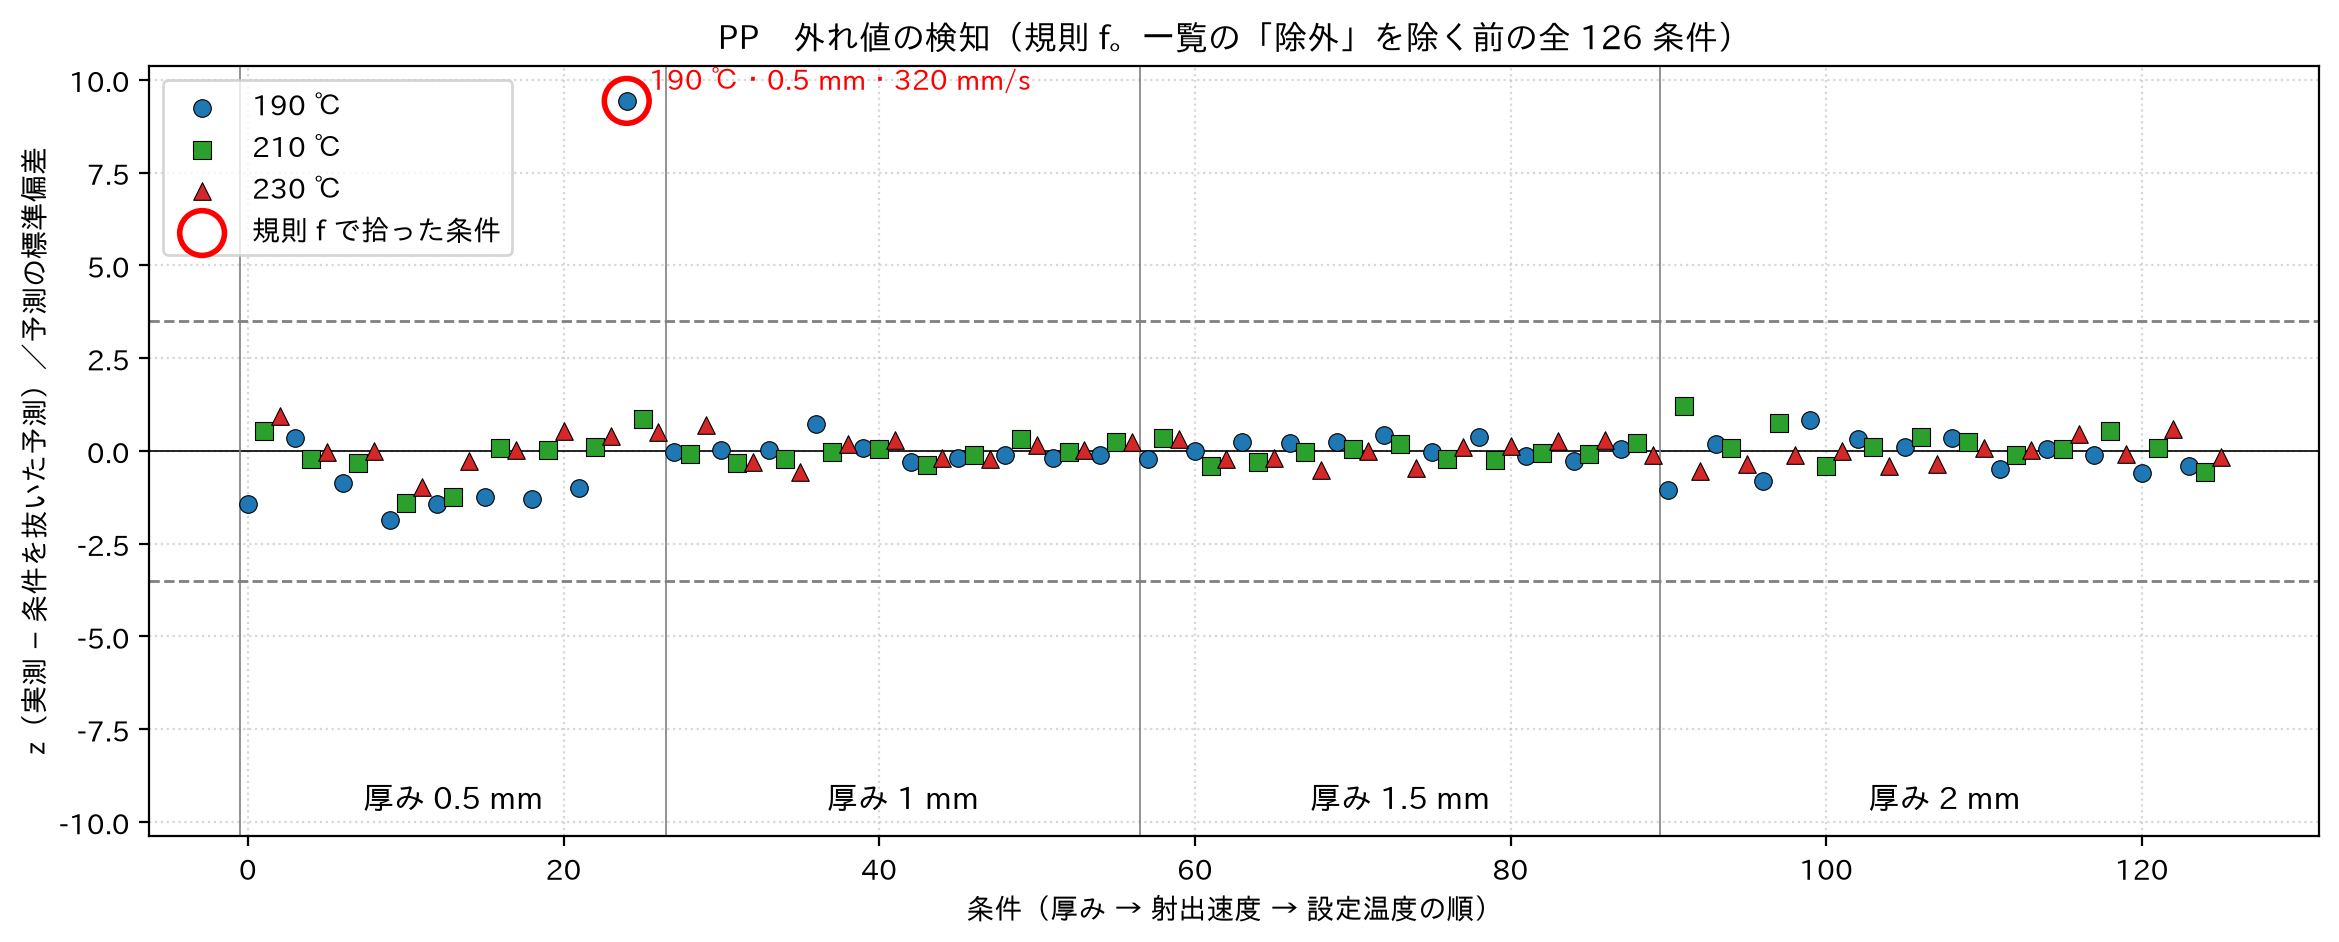
\includegraphics[width=0.9\linewidth]{01_バージンPP再々実験/01_バージンPP再々実験_学習結果/データ確認/外れ値の検知_規則f.png}
\caption{PP の条件ごとの $z$（除く前の全条件）}
\end{figure}
\begin{points}
\pt{何を示す図か}条件を 1 つずつ抜いて、ほかの条件から予測したときの、実測との差の大きさ（$z$）を、条件ごとに並べた図です（ファイル：\file{データ確認/外れ値の検知_規則f.png}）。
\pt{軸と記号}横軸は条件（厚み → 射出速度 → 設定温度の順）、縦軸は $z$。色と形は設定温度。破線が $\pm3.5$。赤い丸が、拾った条件。
\pt{見るポイント}破線の外に大きく飛び出す点があるか。
\pt{今回の結果}PP では、190 ℃・0.5 mm・320 mm/s だけが $z=9.4$ と大きく外れ、問題データ一覧の P03 として除きました。ほかの点は、ほぼ $\pm3$ の中です。粉砕材混合 PP と GPPS は、拾った条件がありません。
\end{points}

\subsection{図2：P3\_3 の性質}
\begin{figure}[H]
\centering
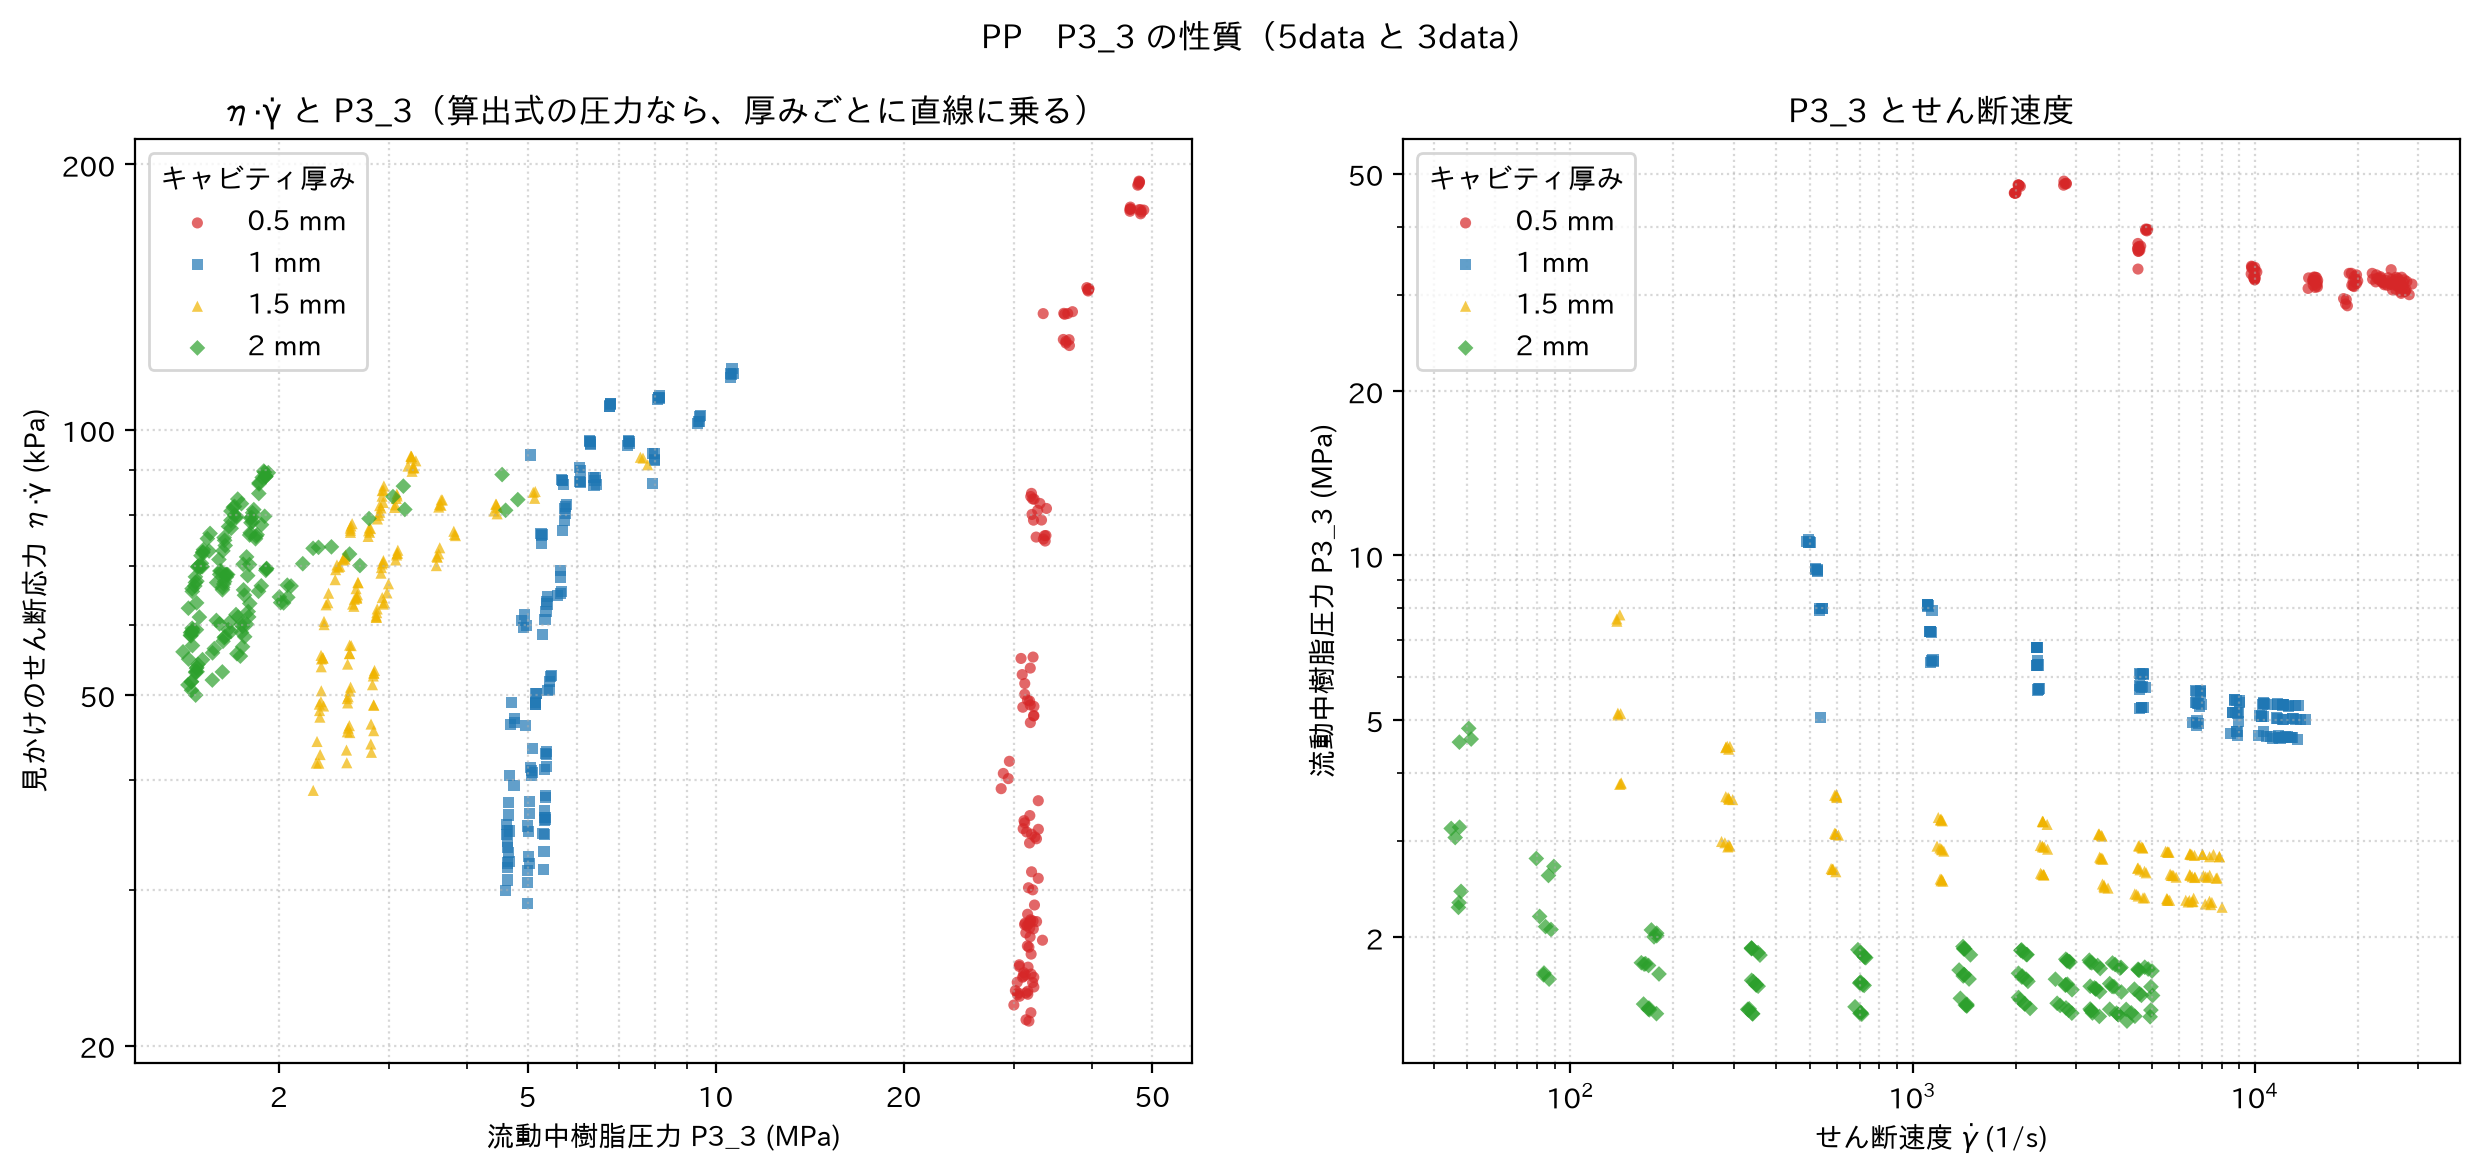
\includegraphics[width=0.9\linewidth]{01_バージンPP再々実験/01_バージンPP再々実験_学習結果/データ確認/P3_3の性質.png}
\caption{左：見かけのせん断応力 $\eta\gd$ と \PIII、右：\PIII\ とせん断速度（色は厚み）}
\end{figure}
\begin{points}
\pt{何を示す図か}\PIII\ が、粘度の算出式の圧力（リークになる量）かどうかを見る図です（ファイル：\file{データ確認/P3_3の性質.png}）。
\pt{軸と記号}どちらも両対数。左の縦軸は $\eta\gd$（kPa）、横軸は \PIII（MPa）。右の横軸はせん断速度、縦軸は \PIII。
\pt{見るポイント}算出式の圧力なら、左の図で、厚みごとに点が 1 本の直線に乗る。
\pt{今回の結果}点は直線に乗らず、算出式の形で表すと誤差は最大 265\%（粉砕材混合 PP 154\%、GPPS 166\%）でした。\PIII\ は算出式の圧力ではありません。右の図のとおり、\PIII\ はせん断速度と厚みでほぼ決まり（厚みが薄いほど大きい）、ln \PII\ との相関は 0.95（PP）と、本体で調べた \PII\ に近い量です。\PIII\ は、流れの結果として測られる量で、成形の前には分かりません。
\end{points}

\subsection{図3：プロファイル尤度（PP・B\_Tset・ショットごとの入力）}
\begin{figure}[H]
\centering
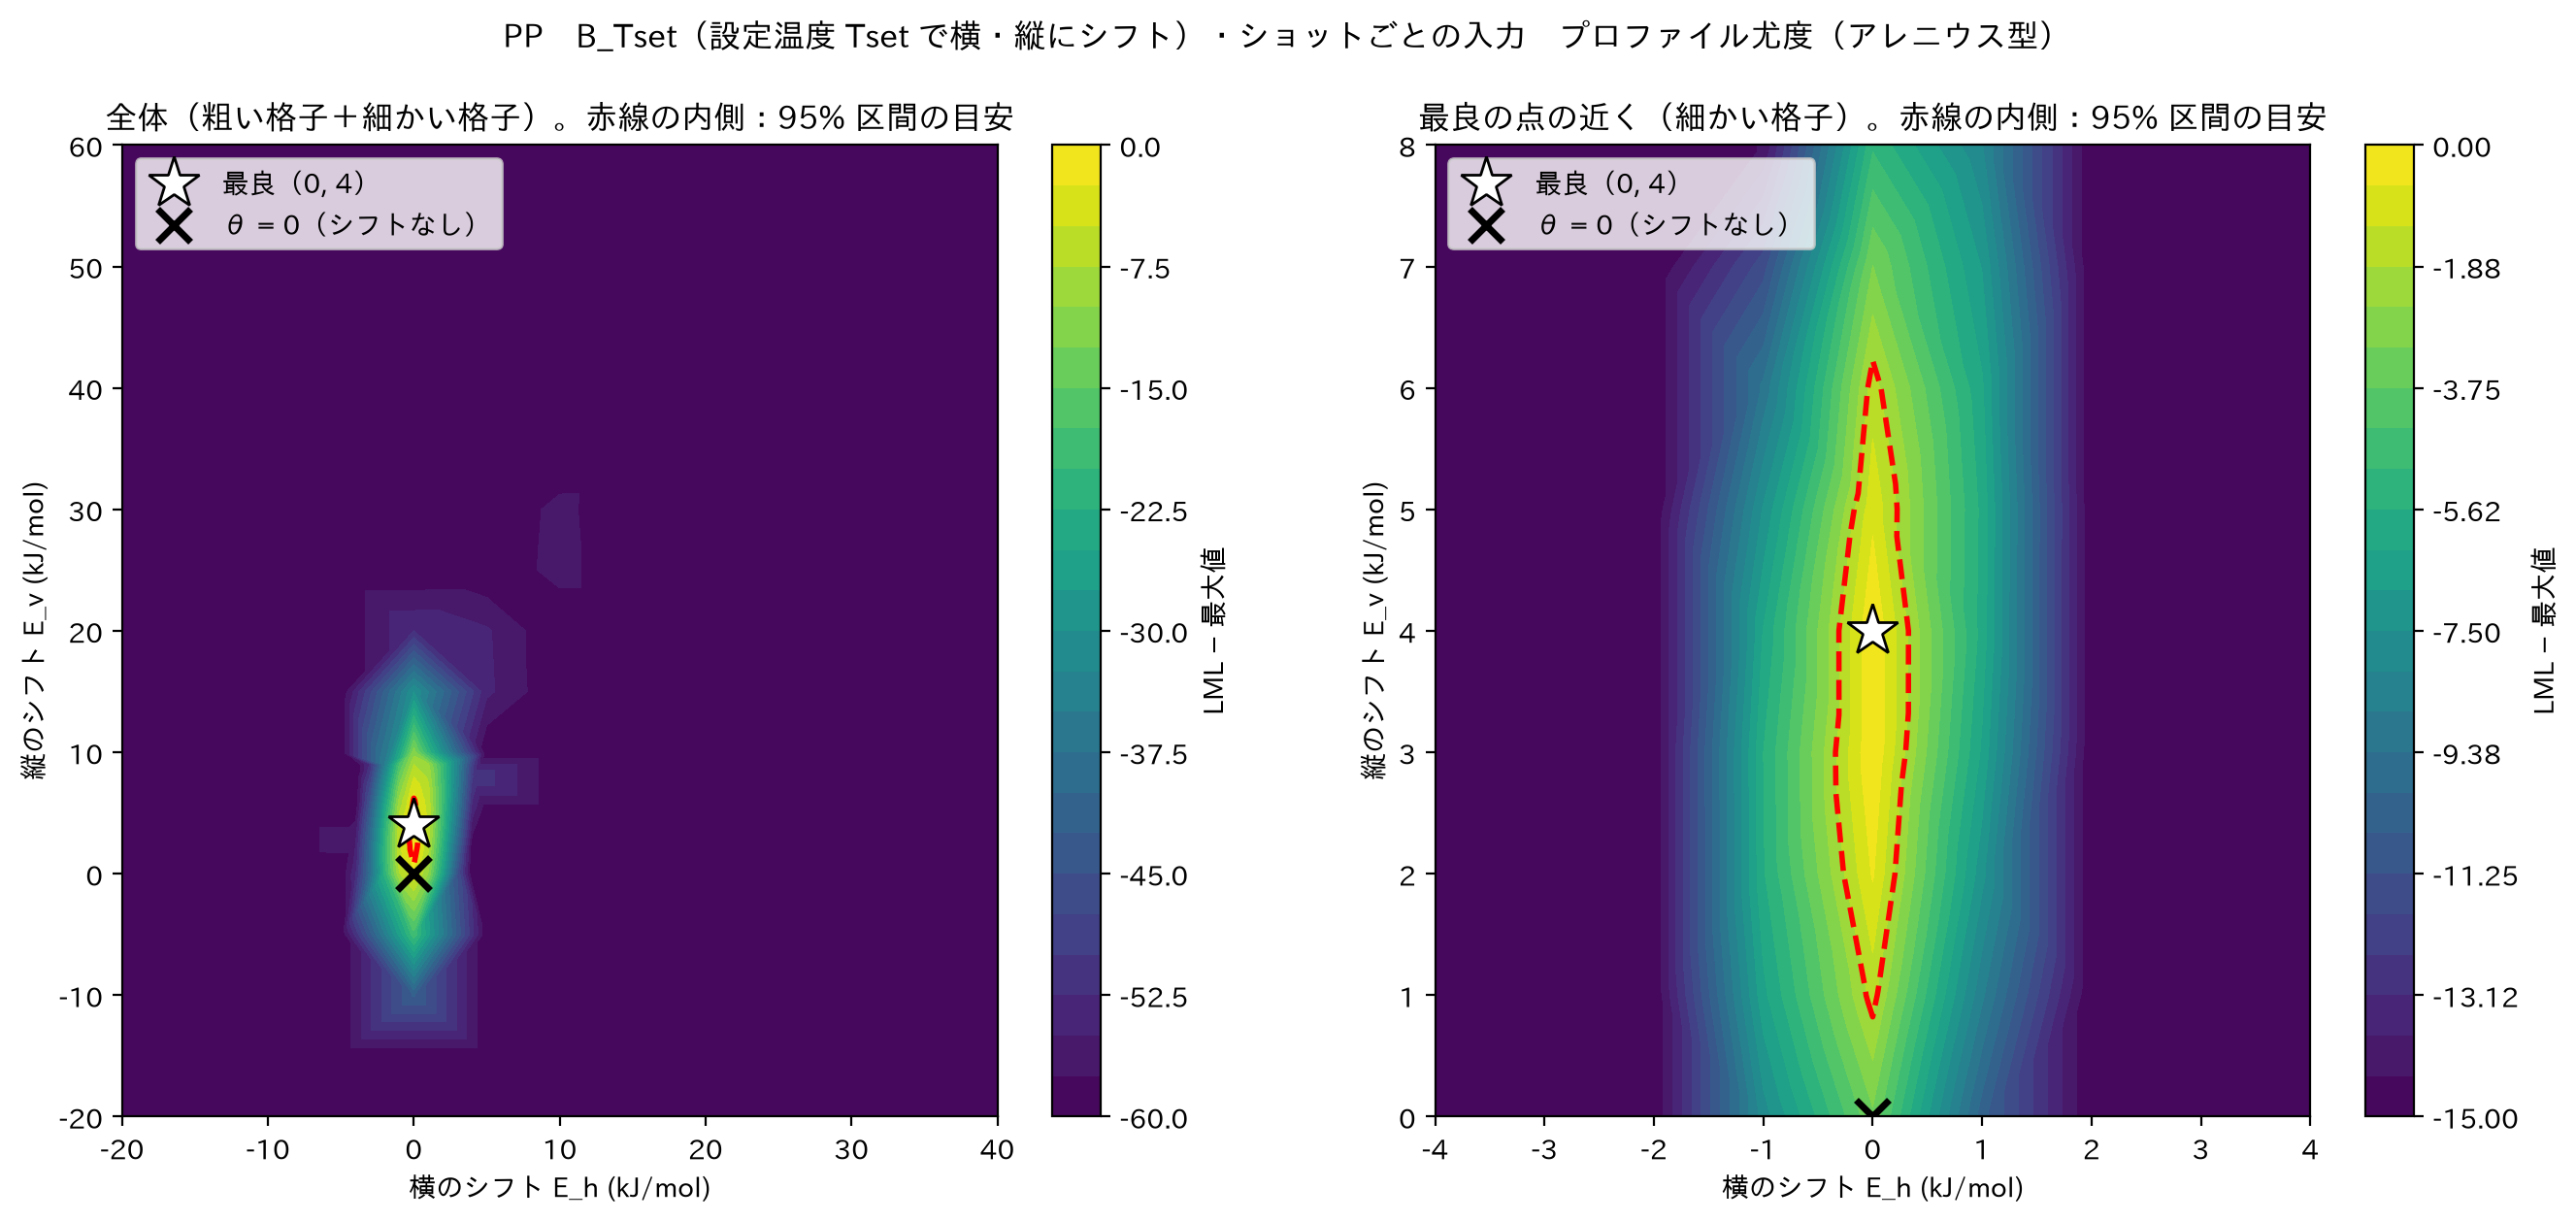
\includegraphics[width=1.0\linewidth]{01_バージンPP再々実験/01_バージンPP再々実験_学習結果/ショットごとの入力/B_Tset/プロファイル尤度.png}
\caption{横のシフト $\Eh$ と縦のシフト $\Ev$ の尤度の面（左：全体、右：最良の点の近く）}
\end{figure}
\begin{points}
\pt{何を示す図か}シフトファクターの係数 $(\Eh,\Ev)$ を格子で振り、それぞれでデータへの合い具合（LML）を求めた図です（ファイル：\file{ショットごとの入力/B_Tset/プロファイル尤度.png}。他のモデル・材料・入力の取り方も同じ名前）。
\pt{軸と記号}横軸が $\Eh$、縦軸が $\Ev$（kJ/mol）。色は LML − 最大値（明るいほどよく合う）。赤線の内側が、おおよその 95\% 区間。★ が最良、× が $\theta=0$（シフトなし）。
\pt{見るポイント}赤線の内側が狭いか（係数がよく決まるか）。斜めに伸びているか（尾根）。× が赤線の外にあるか（シフトを入れた効果があるか）。
\pt{今回の結果}最良は $\Eh=0$、$\Ev=4$ kJ/mol で、横のシフトは 0（ずらさない）になりました。念入りに最適化した $\theta=0$ との LML の差（$\Delta$LML）は 3.2 で、基準の 3.0 を超えます。B\_Tff の $\Delta$LML は 1.1 で、基準に届きません（5.1 節の表）。条件平均の入力（参考）では逆に、B\_Tff の $\Delta$LML が 8.3、B\_Tset が 1.5 でした。
\end{points}

\subsection{図4：シフトファクター（PP・ショットごとの入力）}
\begin{figure}[H]
\centering
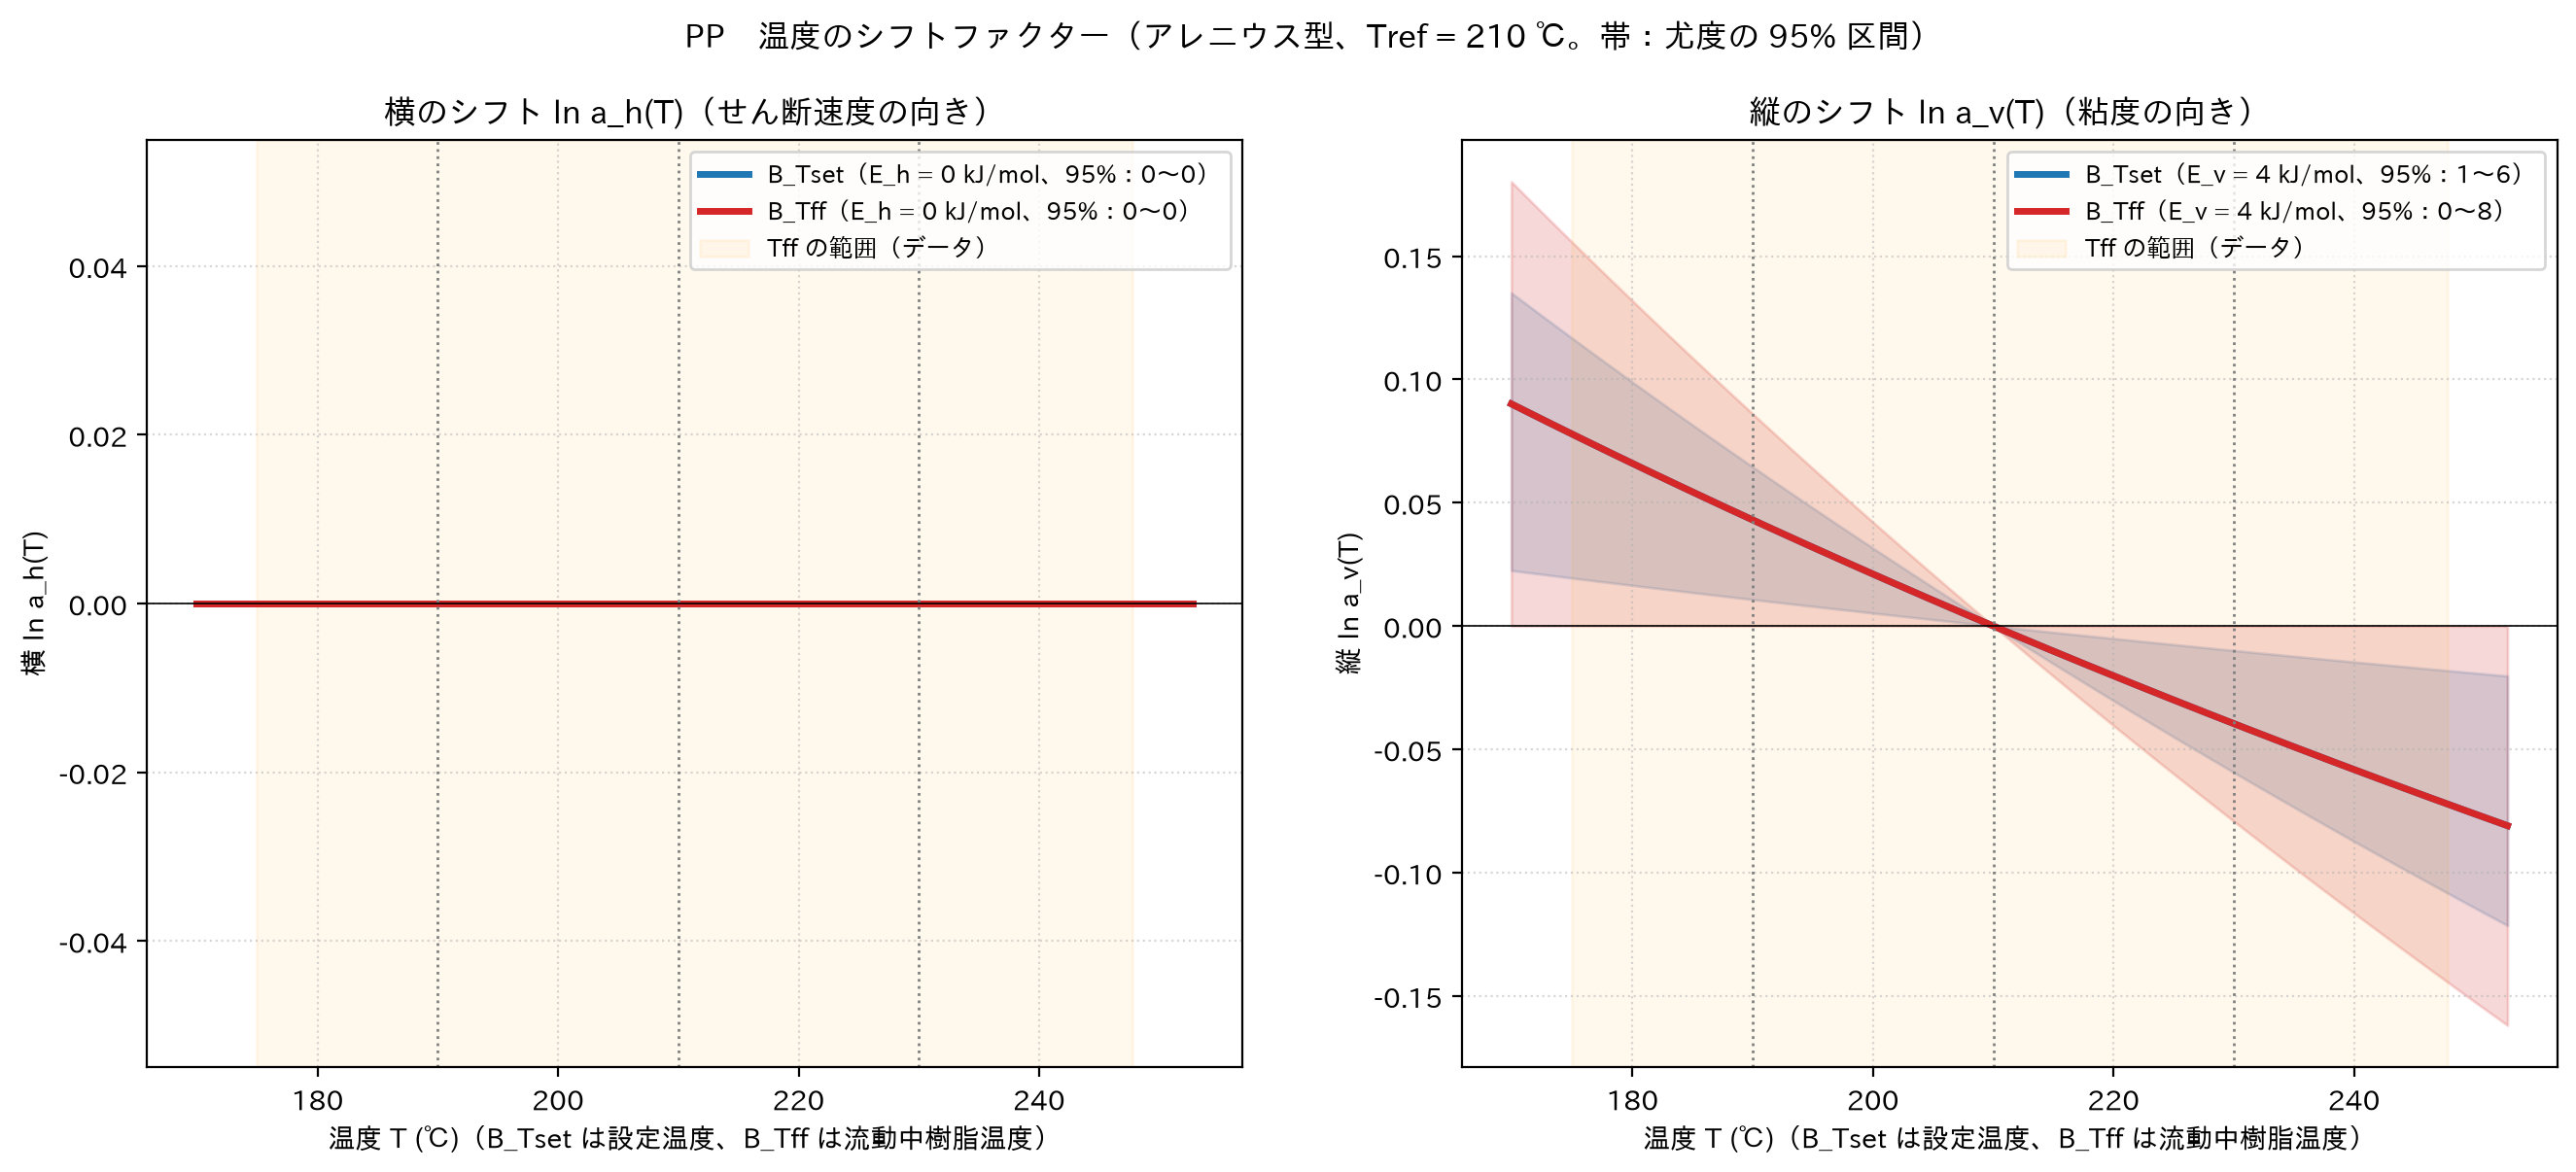
\includegraphics[width=0.9\linewidth]{01_バージンPP再々実験/01_バージンPP再々実験_学習結果/ショットごとの入力/比較/シフトファクター.png}
\caption{横のシフト $\ln a_h(T)$（左）と縦のシフト $\ln a_v(T)$（右）。線が最良、帯が 95\% 区間}
\end{figure}
\begin{points}
\pt{何を示す図か}推定したシフトファクターを、温度の関数として描いた図です（ファイル：\file{<入力>/比較/シフトファクター.png}）。
\pt{軸と記号}横軸が温度（B\_Tset は設定温度、B\_Tff は流動中樹脂温度）。縦軸が $\ln a$。点線は設定温度、薄い橙は $\Tff$ の範囲。$\ln a_v>0$ は、その温度で、同じせん断速度の粘度が $T_{\mathrm{ref}}$ より高いこと。
\pt{見るポイント}線の傾き（温度による変化の大きさ）と、帯の幅（決まり方）。右肩下がりなら「低温ほど粘い」。
\pt{今回の結果}横のシフトは 0（線が水平）で、縦のシフトだけが右肩下がり（低温ほど粘い）です。PP の 190 ℃ と 230 ℃ の縦の倍率 $a_v(190)/a_v(230)$ は、B\_Tset で 1.09、B\_Tff で 1.09 です。5.1 節の表に、全材料・全モデルの値をまとめました。
\end{points}

\subsection{図5：マスターカーブ（PP・B\_Tset・ショットごとの入力）}
\begin{figure}[H]
\centering
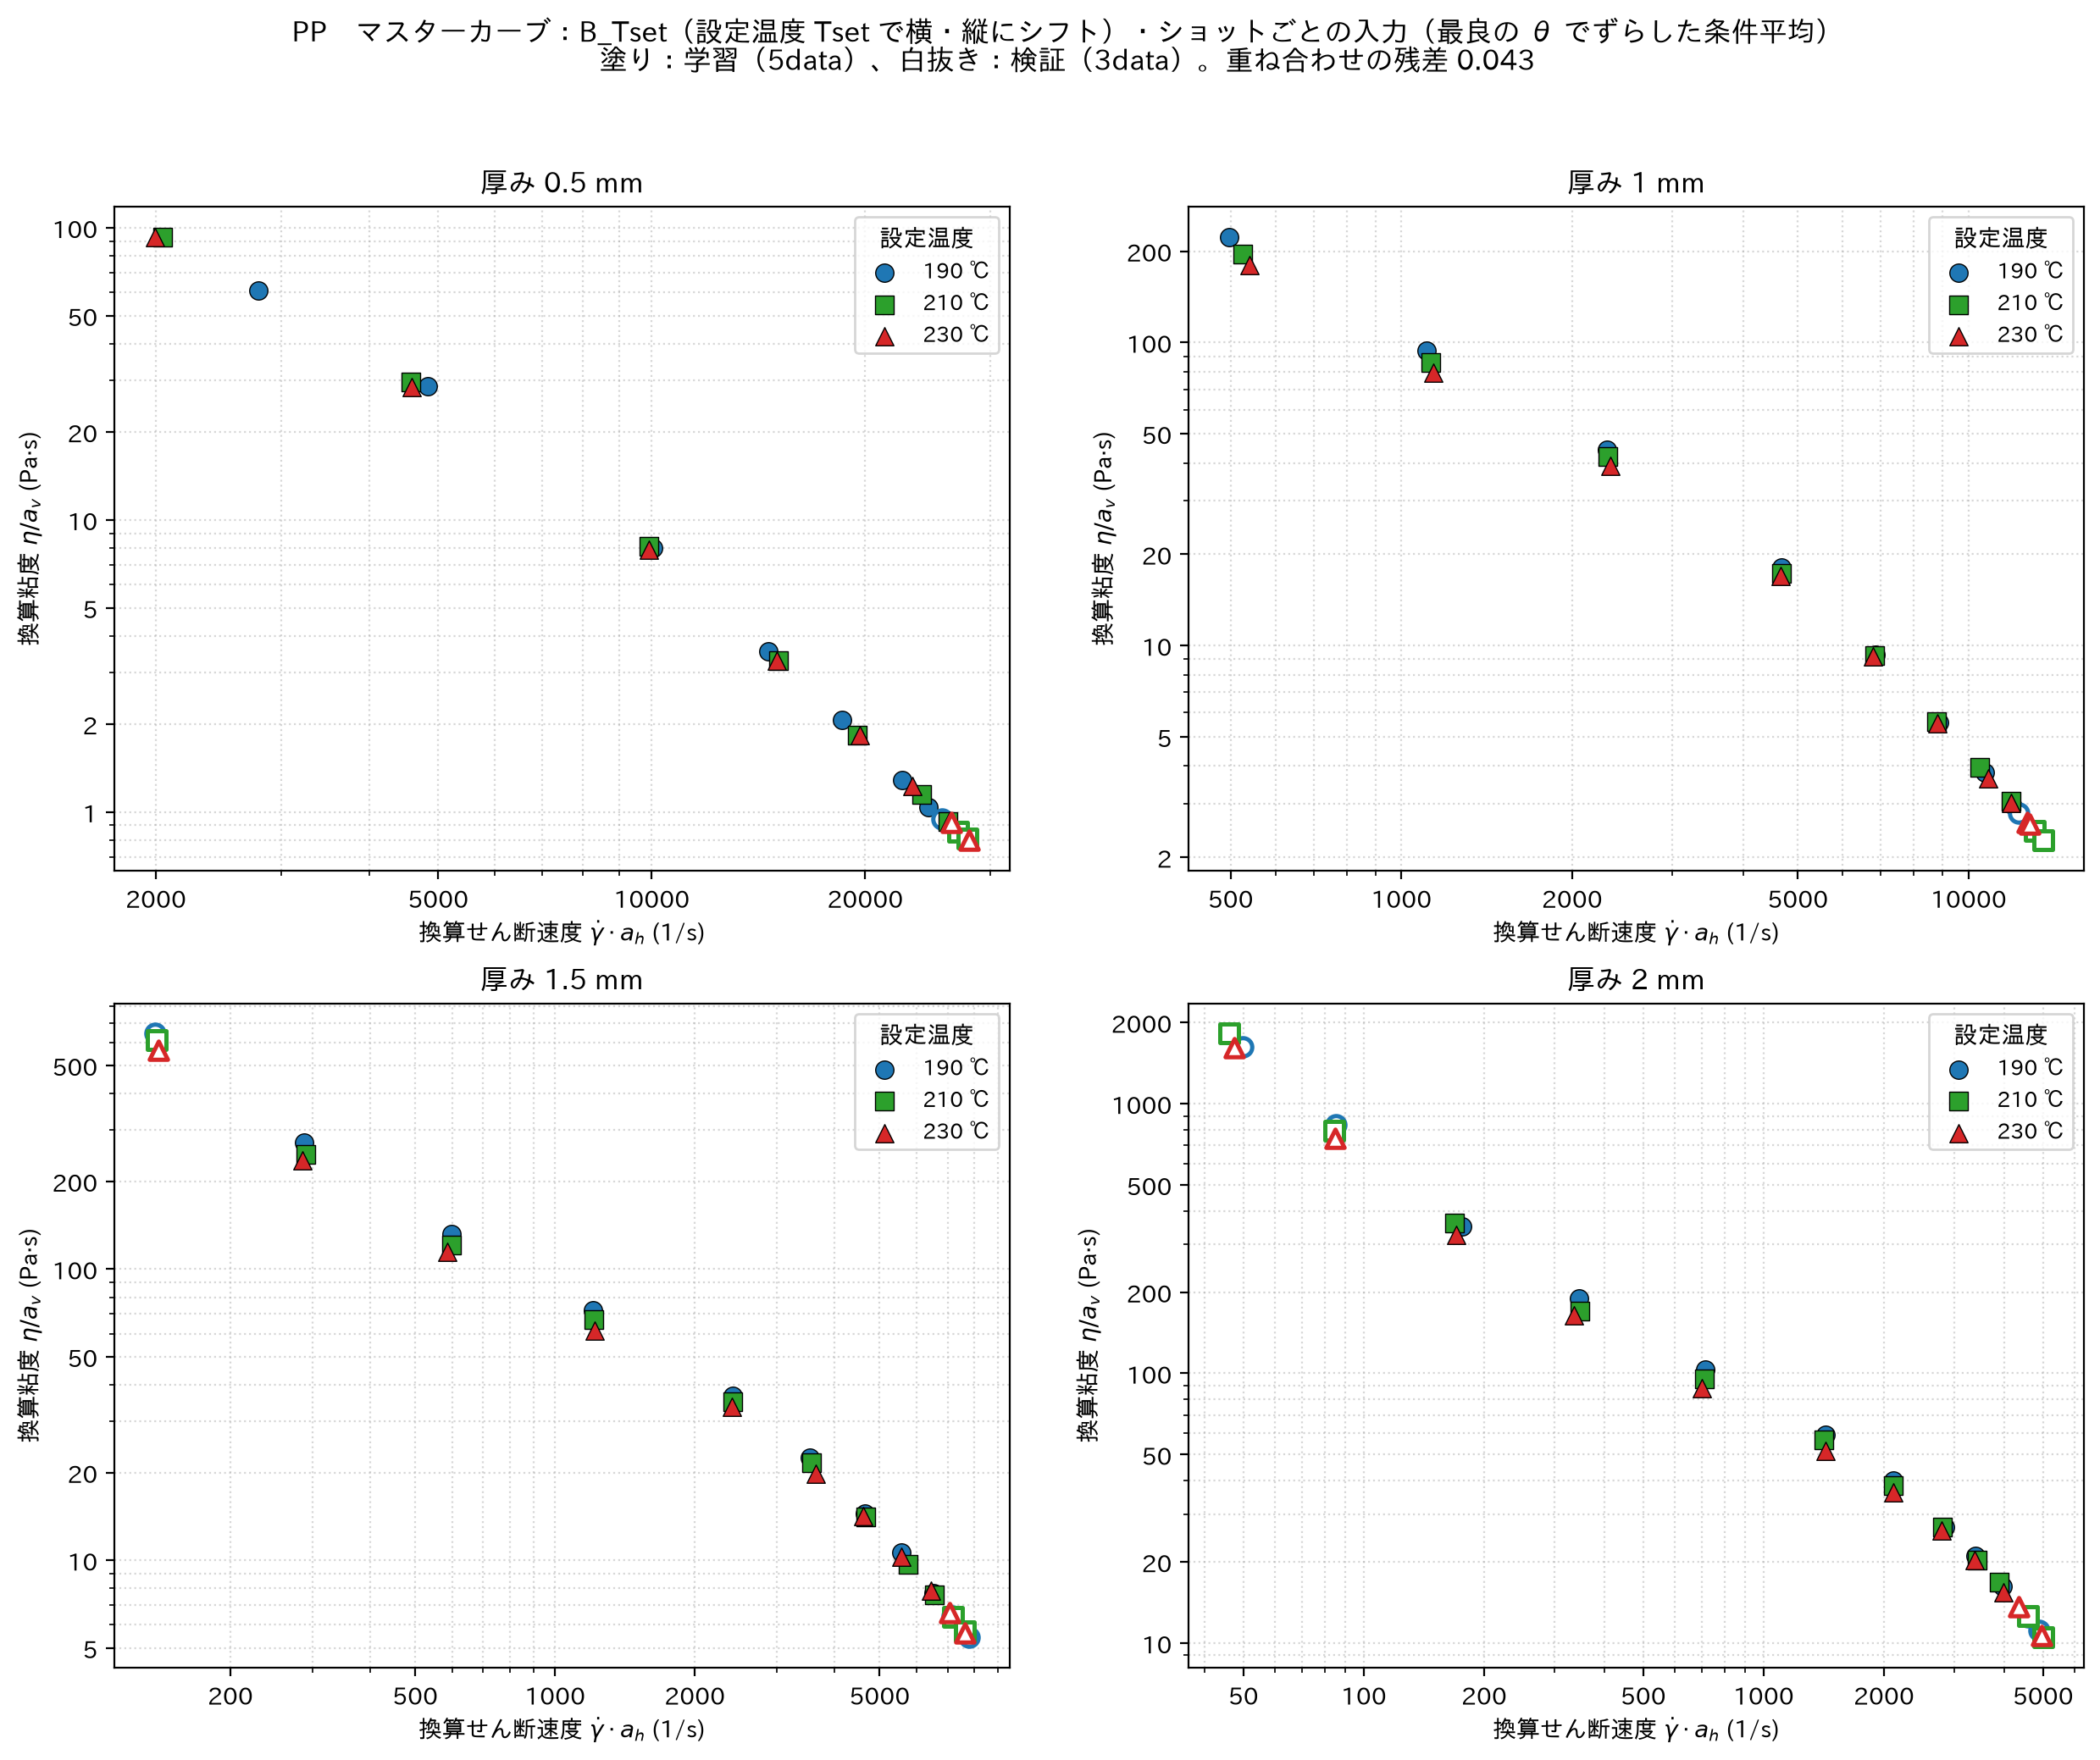
\includegraphics[width=0.9\linewidth]{01_バージンPP再々実験/01_バージンPP再々実験_学習結果/ショットごとの入力/B_Tset/マスターカーブ.png}
\caption{B\_Tset の最良の係数でずらした条件平均の点（厚みごと。シフト前は \file{比較/流動曲線_シフト前.png}）}
\end{figure}
\begin{points}
\pt{何を示す図か}温度ごとの曲線を、シフトファクターでずらして重ねた図です（ファイル：\file{ショットごとの入力/B_Tset/マスターカーブ.png}）。点は、見やすさのため成形条件ごとの平均です。
\pt{軸と記号}横軸が換算せん断速度 $\gd a_h$、縦軸が換算粘度 $\eta/a_v$（両対数）。色が設定温度。塗りが学習、白抜きが検証。
\pt{見るポイント}温度の違う点が、1 本の曲線に重なるか。図の上の「重ね合わせの残差」が、シフト前より小さいか。
\pt{今回の結果}PP の B\_Tset で、重ね合わせの残差は 0.067 → 0.043 に減り、温度ごとの点が 1 本の曲線に近づきました。B\_Tff では 0.067 → 0.044 です（5.1 節の表）。
\end{points}

\subsection{図6：せん断速度 ― 粘度の学習結果（PP・厚み 2.0 mm。ショットごとの入力）}
\begin{figure}[H]
\centering
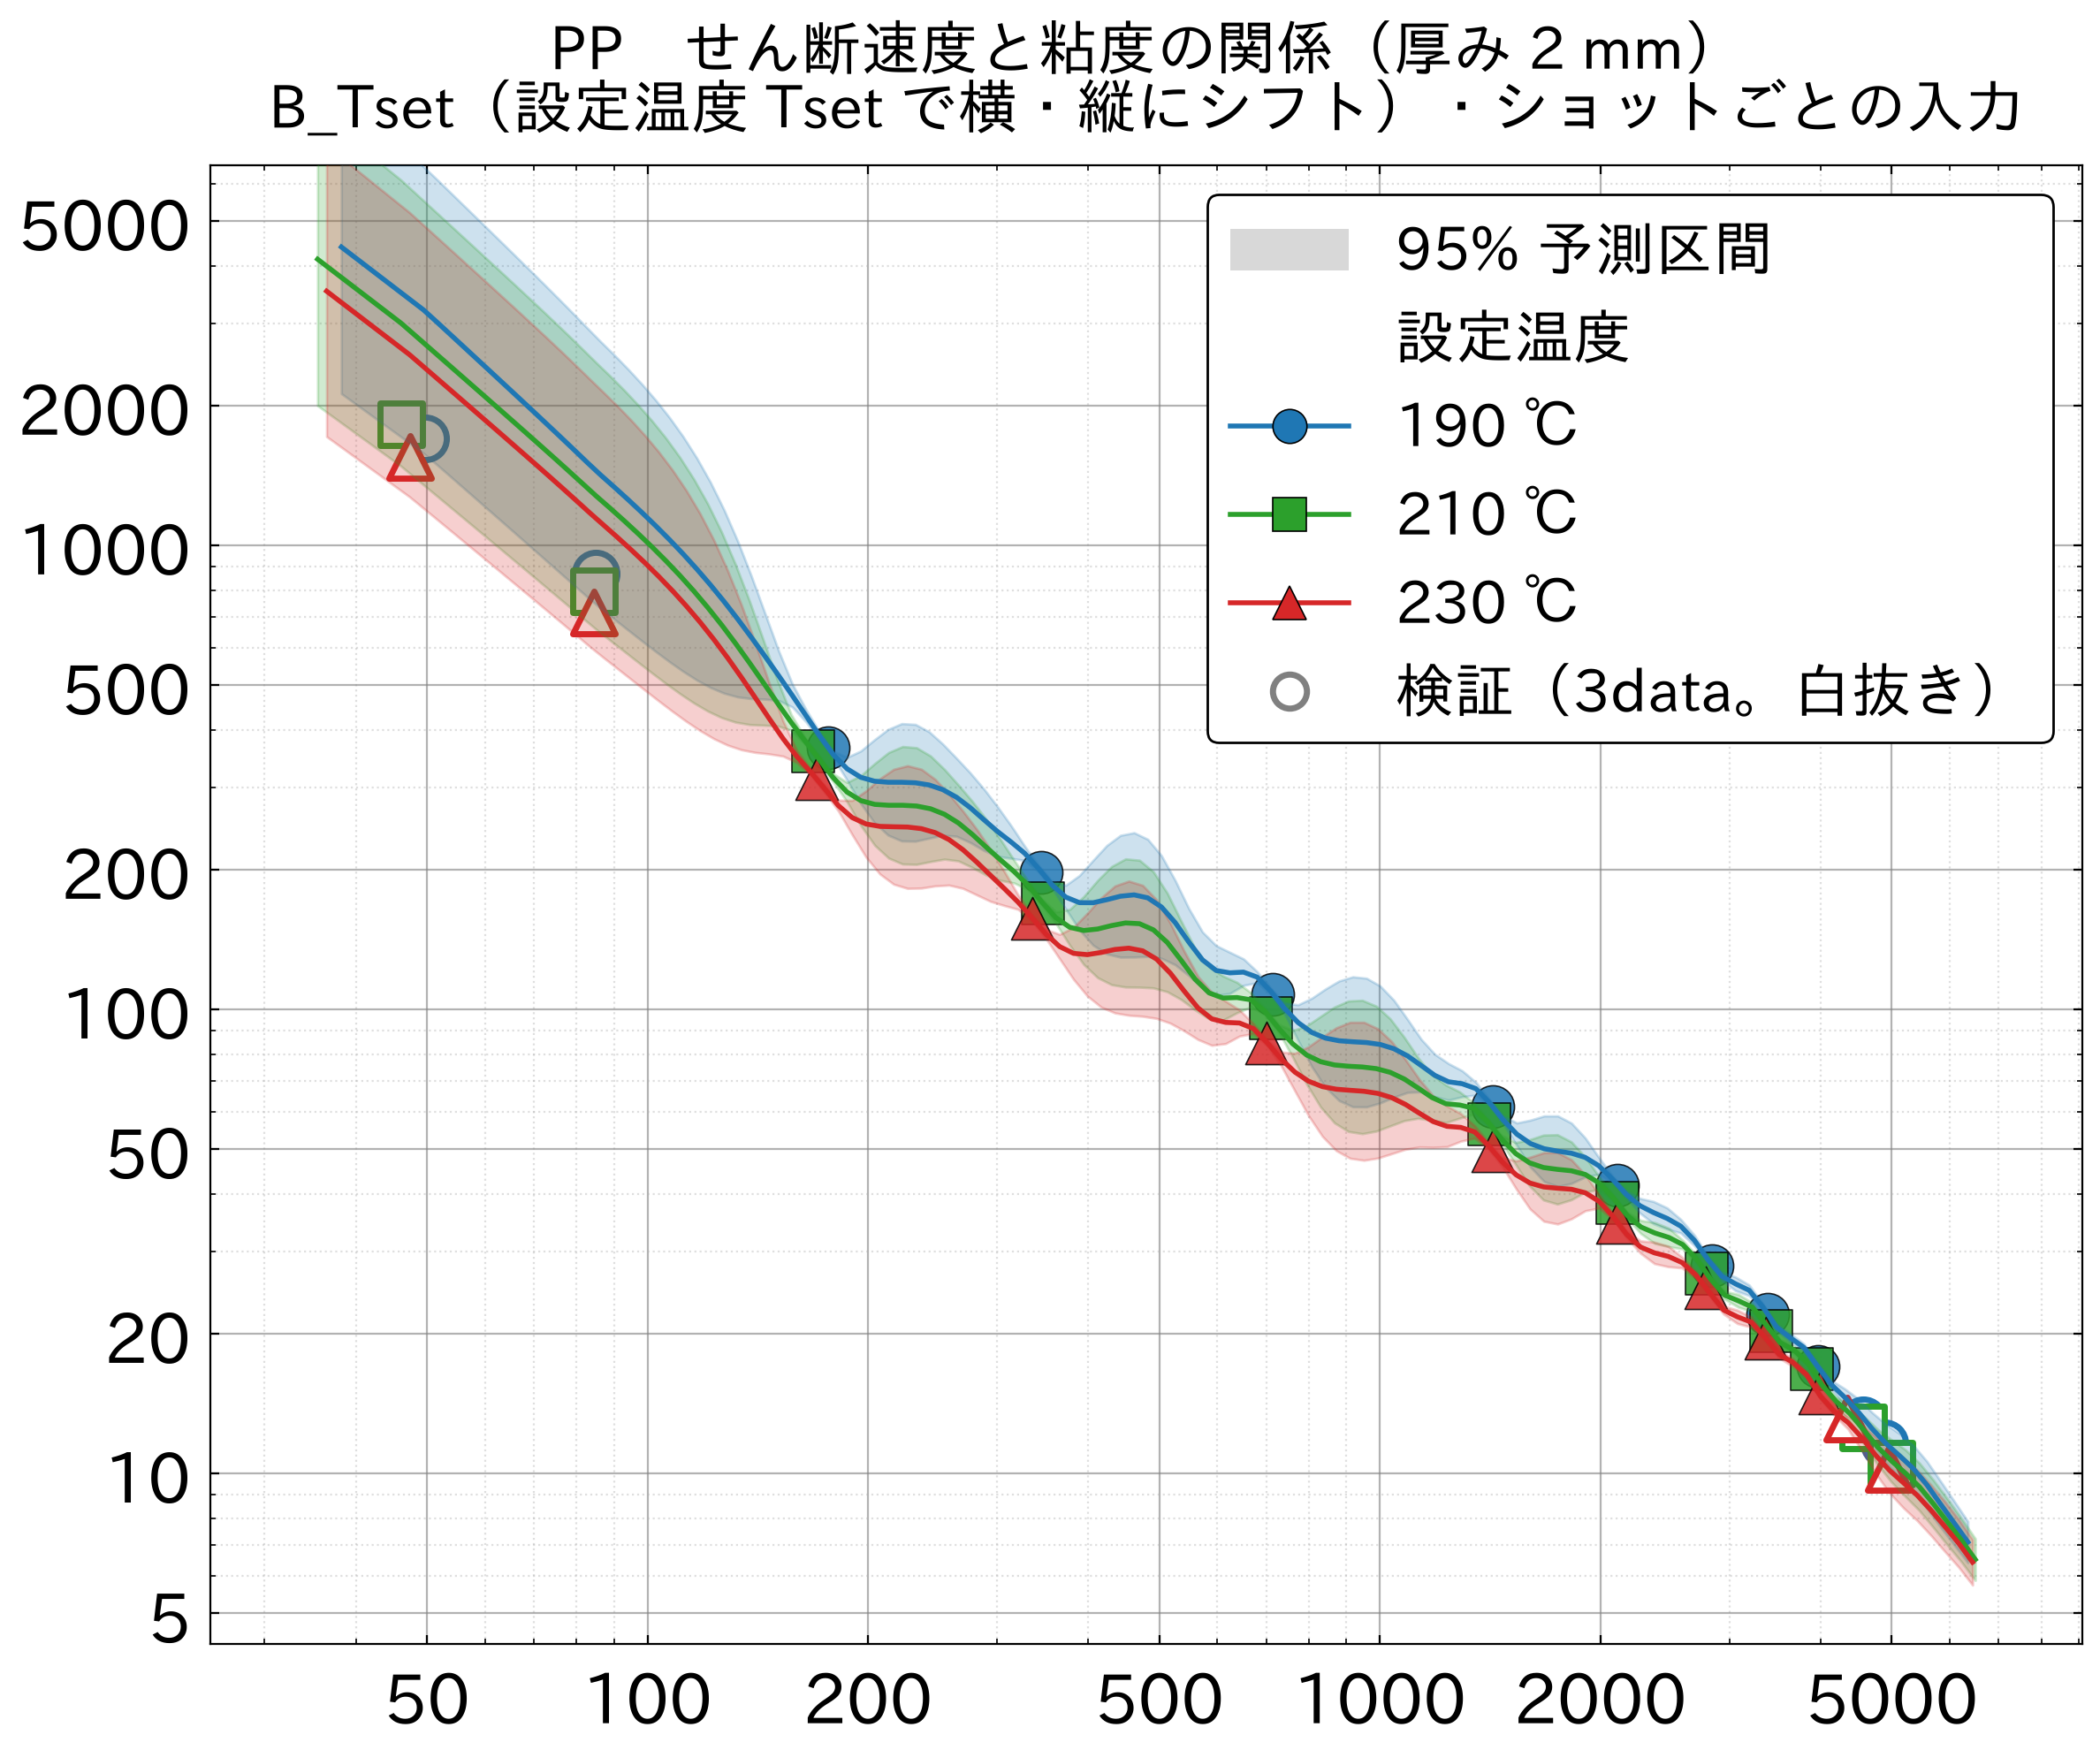
\includegraphics[width=0.9\linewidth]{01_バージンPP再々実験/01_バージンPP再々実験_学習結果/ショットごとの入力/B_Tset/せん断速度_粘度/せん断速度_粘度_厚みごと_2mm.png}
\caption{B\_Tset の予測曲線と 95\% 予測区間（色が設定温度）}
\end{figure}
\begin{points}
\pt{何を示す図か}6月のノートのセル9-2 と同じ見せ方の図です（ファイル：\file{<入力>/<モデル>/せん断速度_粘度/}。設定温度ごと・厚みごと・全厚み共通の図があります）。
\pt{軸と記号}横軸がせん断速度、縦軸が粘度（両対数）。線が予測の平均、帯が 95\% 予測区間。塗りの点が学習（5data）、白抜きが検証（3data）で、どちらもショットごとの計測値（1 つの成形条件に、ショットの数だけ点があります）。目盛りは、軸の範囲が 2.5 桁以下なら 1・2・5 × $10^n$、それより広いとき（または目盛りの数字が重なるとき）は $10^n$ だけです（10 月 26 日から。この図は両軸とも $10^n$）。
\pt{見るポイント}白抜きの点（学習していない低速側・高速側）が、線の近く・帯の中にあるか。曲線が滑らかか。
\pt{今回の結果}ショットごとの入力では、曲線が条件の間で細かく波打ち、低速側（左端の白抜き）の予測は実測から外れやすくなります（PP の B\_Tset の低速側の RMSE：ショットごと 0.447、条件平均 0.083）。ショットごとの $\gd$ には、同じ条件の中のゆれ（センサへの到達時刻のゆれ。$\ln\eta$ と $\ln\gd$ が傾き約 $-2$ で一緒に動く）が入っていて、GP がそれに合わせて、$\ln\gd$ の長さスケールを短くする（C で 0.18。条件平均では 6.4）ためです。次の図7（条件平均の入力）と比べてください。
\end{points}

\subsection{図7：同じ図（条件平均の入力。参考）}
\begin{figure}[H]
\centering
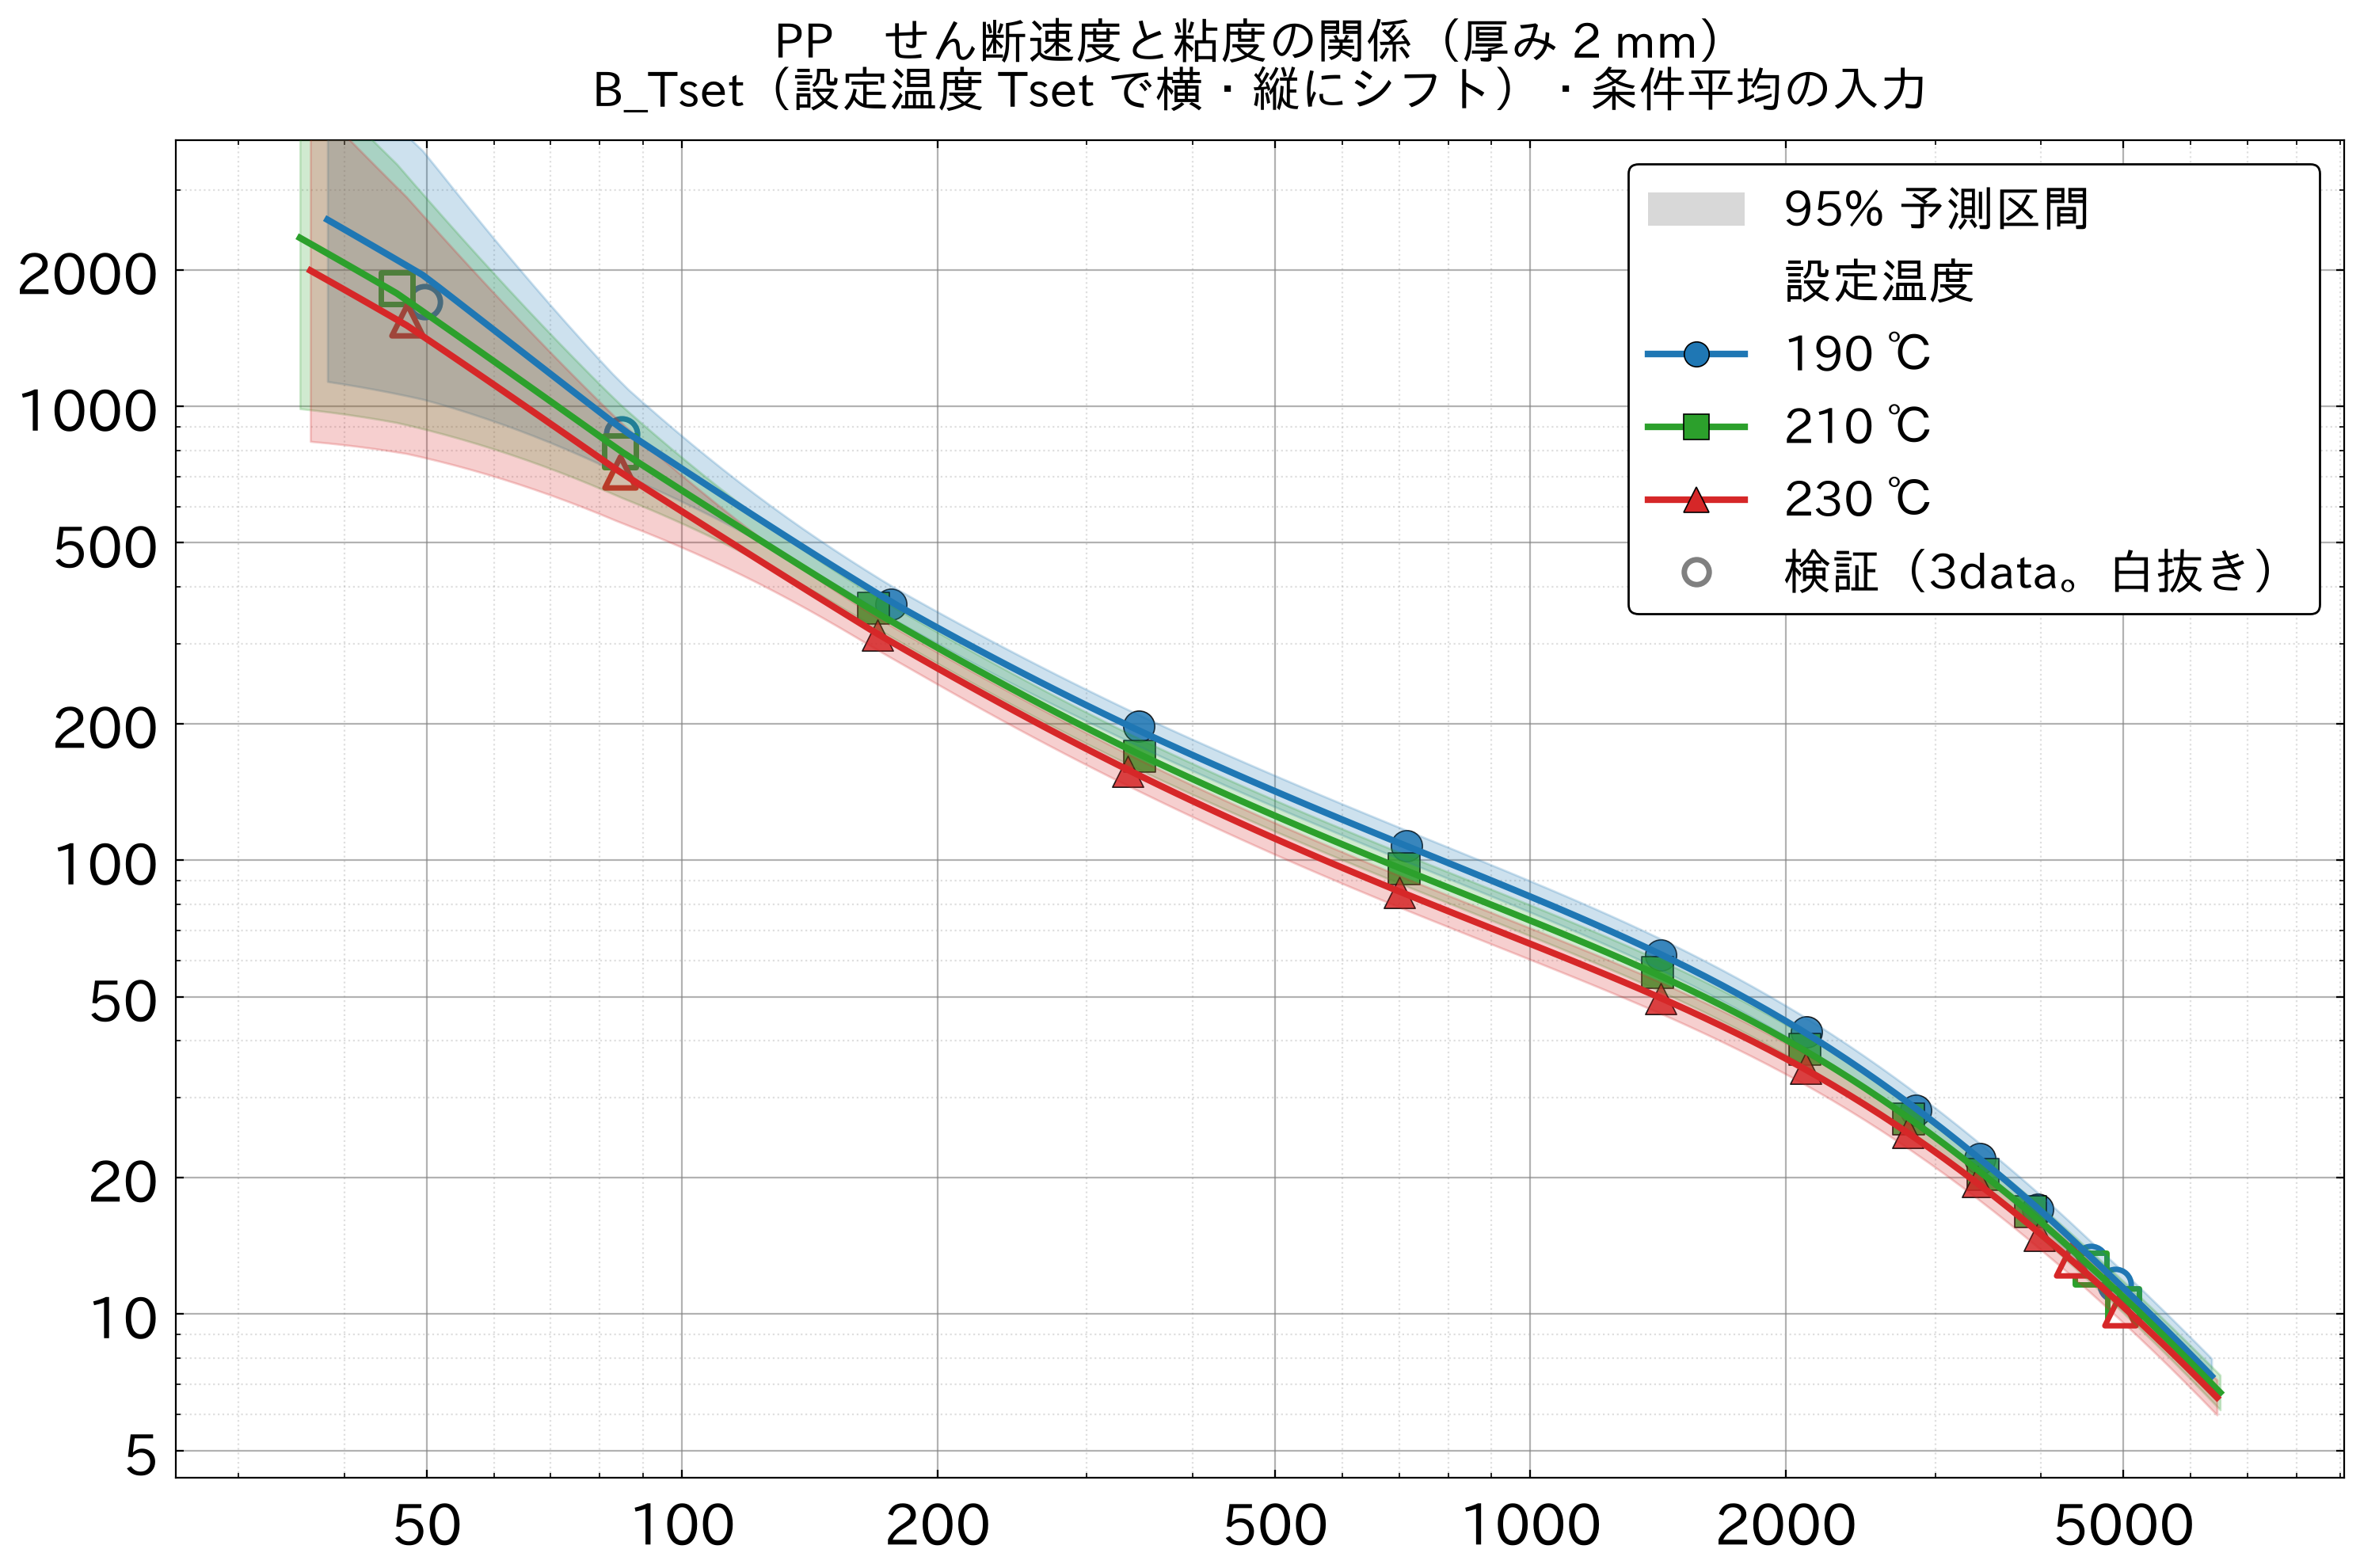
\includegraphics[width=0.9\linewidth]{01_バージンPP再々実験/01_バージンPP再々実験_学習結果/条件平均の入力/B_Tset/せん断速度_粘度/せん断速度_粘度_厚みごと_2mm.png}
\caption{条件平均の入力の B\_Tset（PP・厚み 2.0 mm）}
\end{figure}
\begin{points}
\pt{何を示す図か}図6と同じ図を、条件平均の入力（10 月 15〜22 日の既定）で描いたものです。
\pt{軸と記号}図6と同じ。ただし、点は成形条件ごとの平均です（このときの学習に合わせた点です）。目盛りの付け方は図6と同じです（10 月 26 日に、保存済みのモデルから作り直しました）。
\pt{見るポイント}曲線の形と、低速側の白抜きの点と線のずれ。
\pt{今回の結果}条件平均の入力では、曲線は滑らかで、低速側の点も帯の近くにあります。本体の手順3b で、$\gd$ を条件平均で入れると決めた理由と同じです。10 月 23 日に、ユーザーの決定で、ノートの既定をショットごとに変えました。
\end{points}

\subsection{図8：全厚み共通の平均関数と予測幅（PP・B\_Tset・ショットごとの入力）}
\begin{figure}[H]
\centering
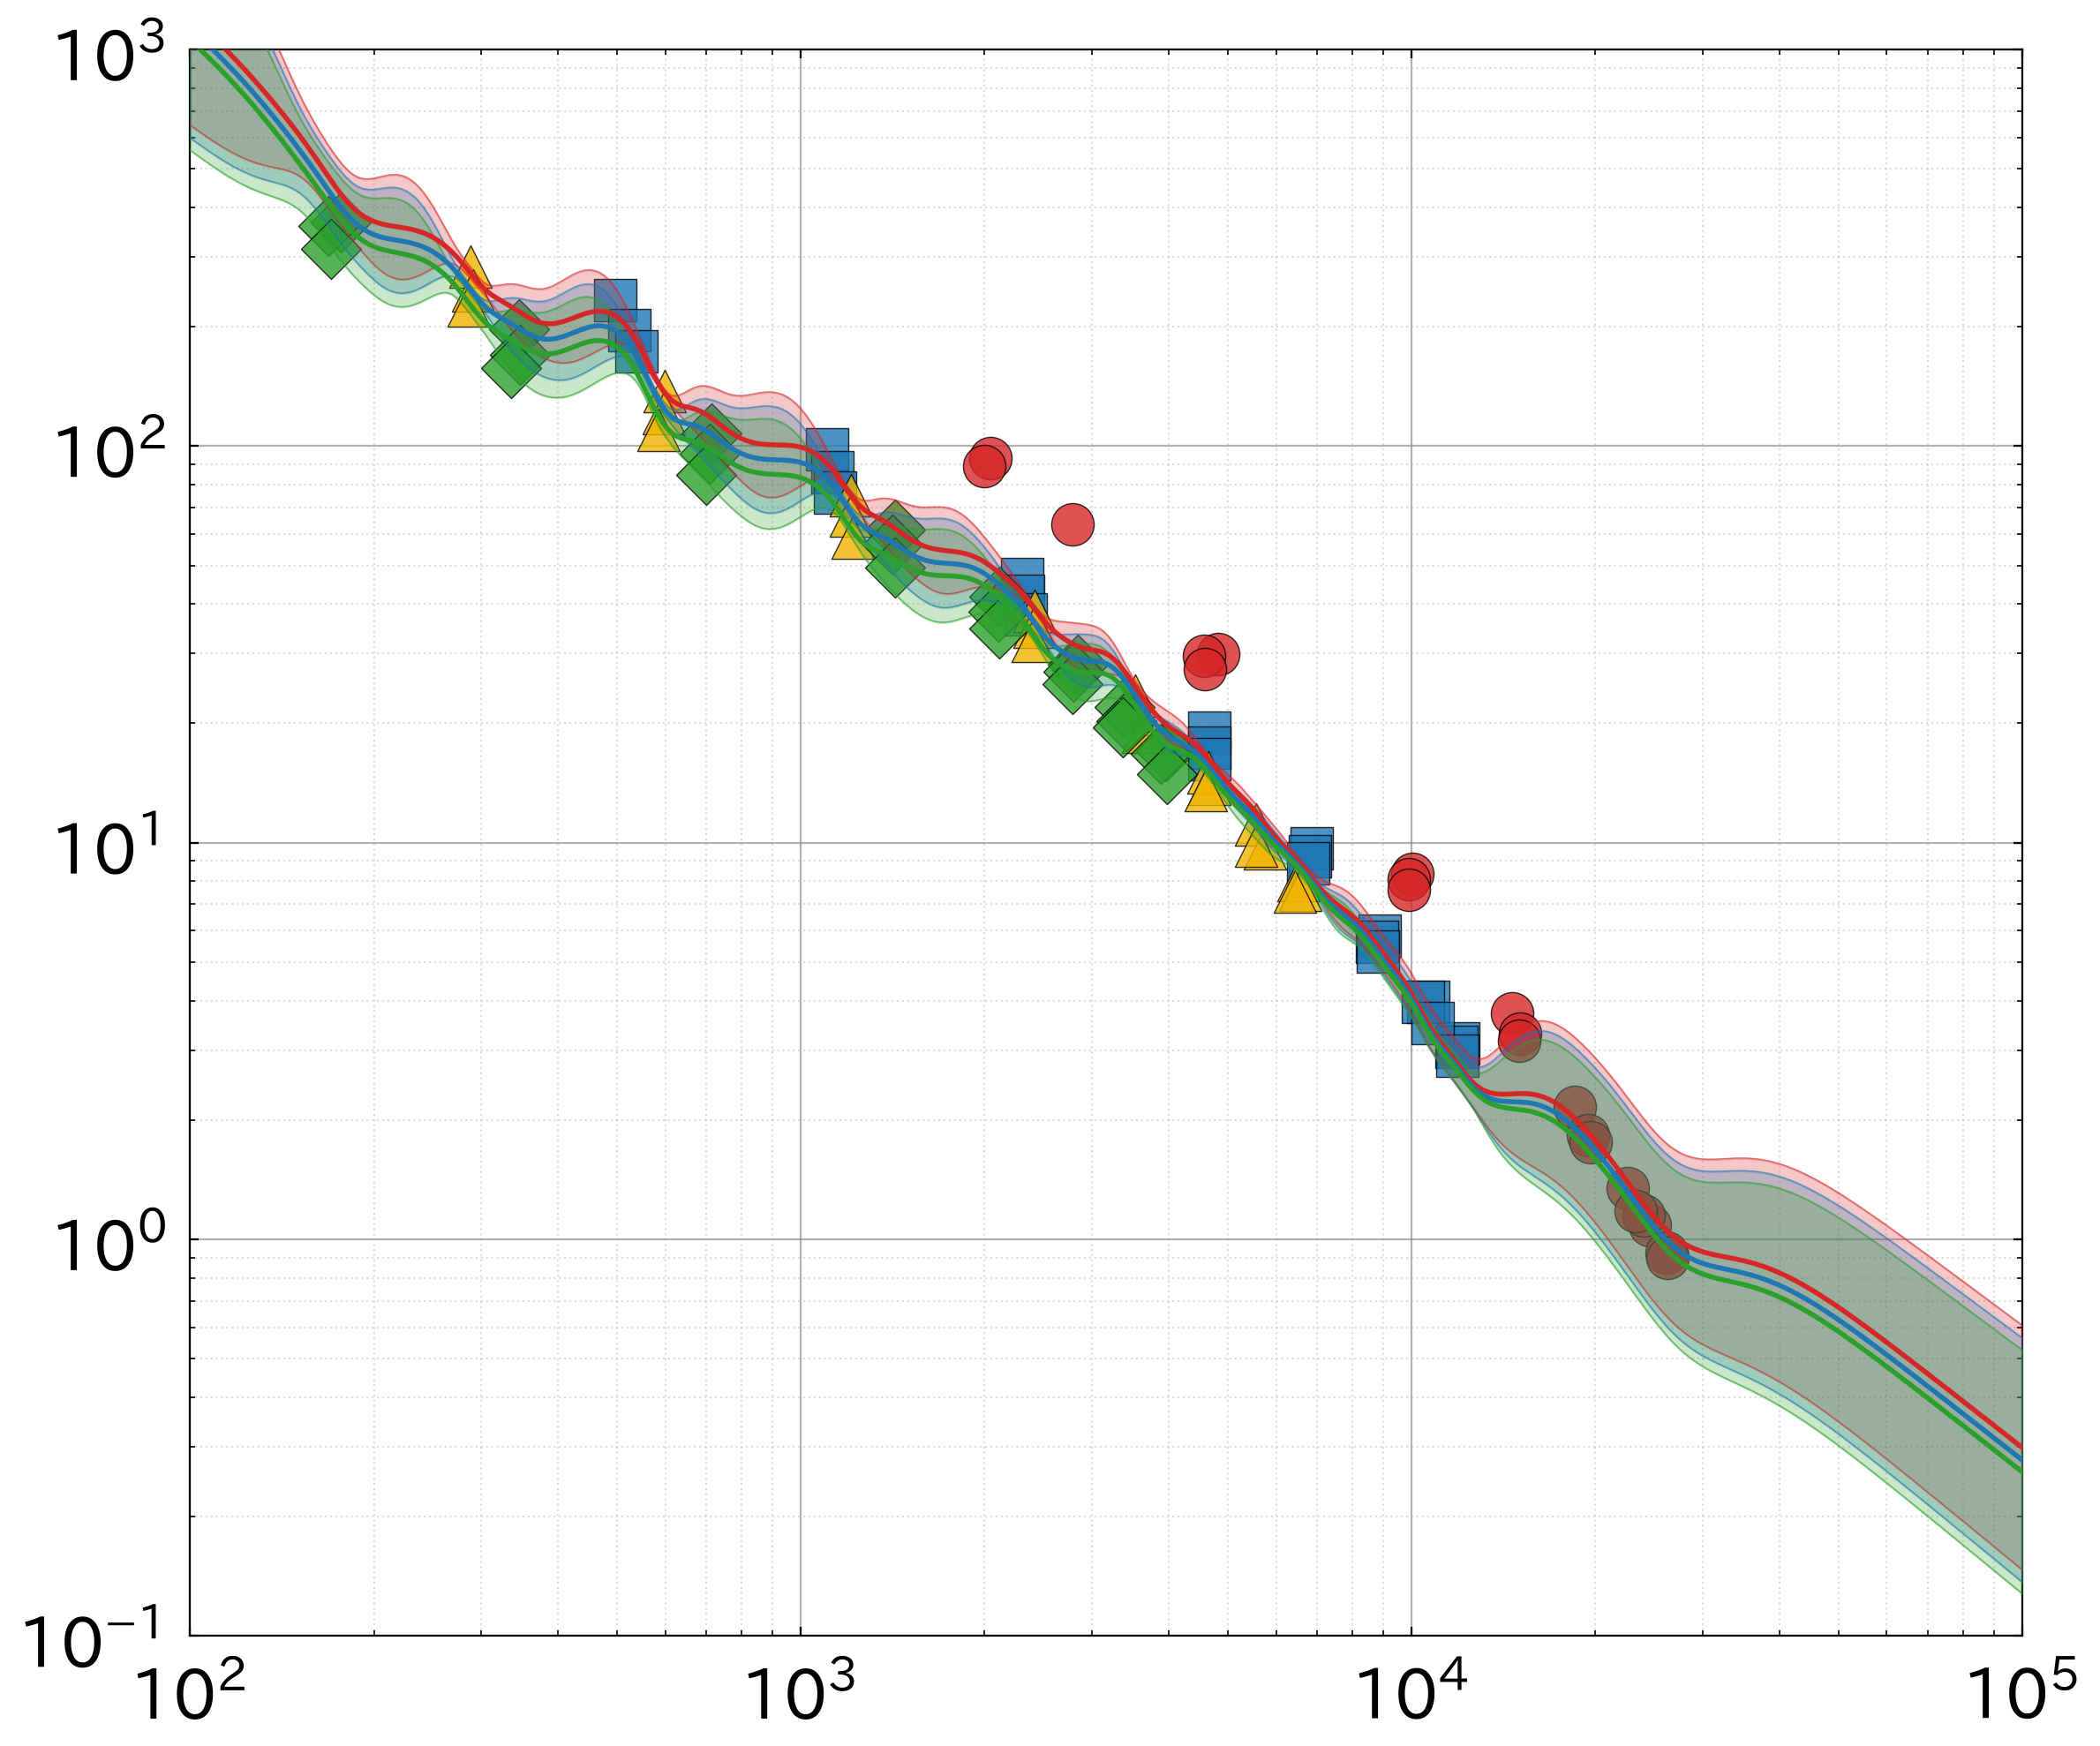
\includegraphics[width=0.62\linewidth]{01_バージンPP再々実験/01_バージンPP再々実験_学習結果/ショットごとの入力/B_Tset/せん断速度_粘度/せん断速度_粘度_全厚み共通_全温度.png}
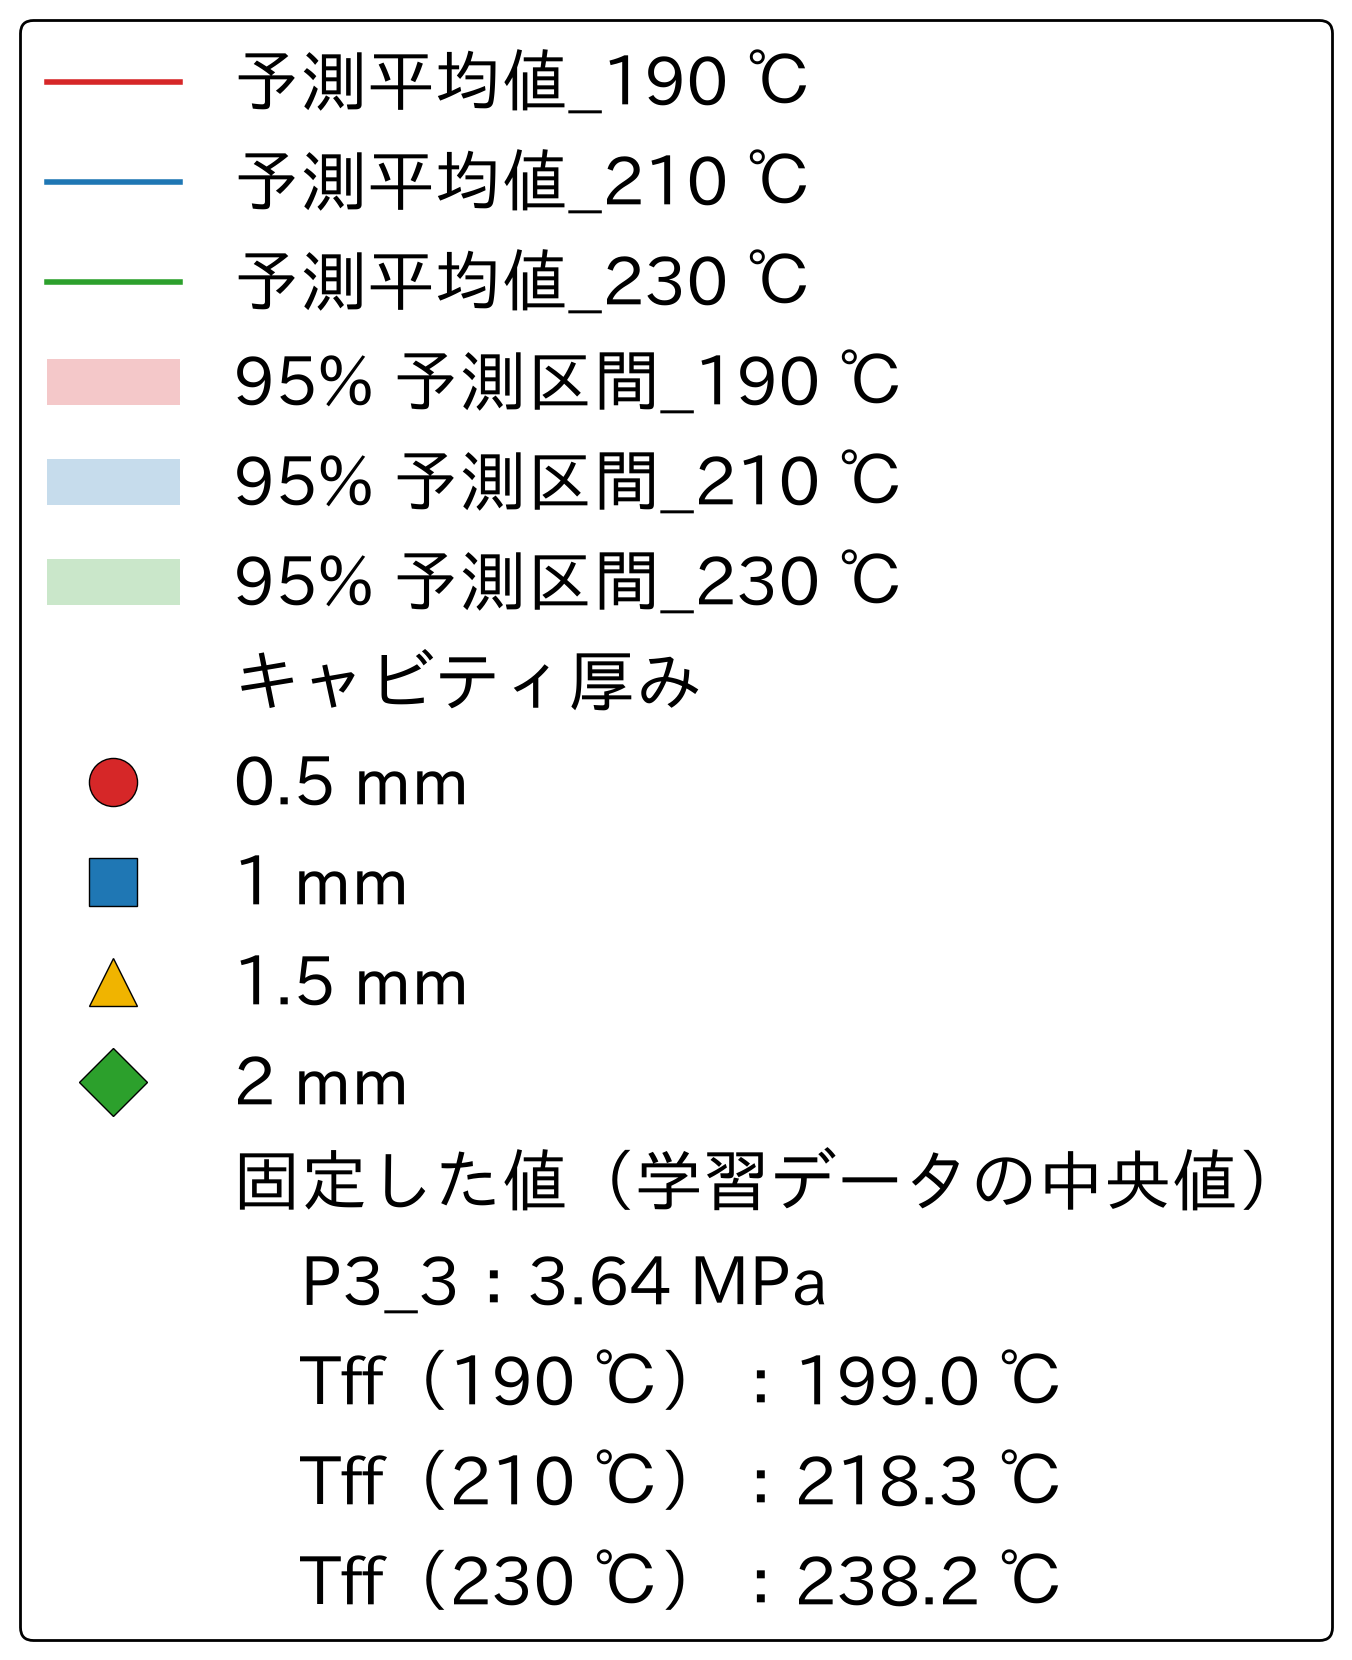
\includegraphics[width=0.3\linewidth]{01_バージンPP再々実験/01_バージンPP再々実験_学習結果/ショットごとの入力/B_Tset/せん断速度_粘度/せん断速度_粘度_全厚み共通_全温度_凡例.png}
\caption{加熱シリンダ温度ごとの、全厚み共通の平均関数と 95\% 予測区間（左：グラフ、右：凡例の画像。線・帯の色は 190 ℃ が赤、210 ℃ が青、230 ℃ が緑）}
\end{figure}
\begin{points}
\pt{何を示す図か}6月のノートのセル9-2 と同じ見せ方で、全キャビティ厚みの学習データの点（ショットごとの計測値。色・形は厚み）を重ね、温度ごとの平均関数と予測幅を、1 つのグラフで比べる図です（ファイル：\file{せん断速度_粘度_全厚み共通_全温度.png} と \file{…_凡例.png}。温度ごとの図 \file{…_全厚み共通_190C.png} なども同じフォルダにあります）。
\pt{軸と記号}両軸とも 10 の累乗の目盛り（6月と同じ）。曲線は、せん断速度だけを動かし、\PIII\ は学習データの中央値、$\Tff$ は、その設定温度の学習データの中央値に固定したもの（固定した値は、凡例の画像に書いてあります）。
\pt{見るポイント}温度ごとの曲線と帯が、どれくらい離れているか。点（厚みごと）が曲線のどちら側に散らばるか。
\pt{今回の結果}\textbf{読むときの注意}：入力が 4 つあるので、1 本の曲線にするには、ほかの入力を固定する必要があります。厚みの違いは \PIII\ を通して入るので、厚み 0.5 mm の点は、共通の曲線の上に離れて並びます。また、温度ごとの曲線の違いには、$\Tset$ の効果と、固定した $\Tff$ の違い（約 20 ℃ ずつ）の両方が入っています。\textbf{この図だけでは、シフトの証拠にはなりません}。シフトの根拠は、図3〜5（尤度、シフトファクター、マスターカーブ）と 5.1 節の表で見ます。
\end{points}

\subsection{図9：3data の予測検証（PP・B\_Tset・ショットごとの入力）}
\begin{figure}[H]
\centering
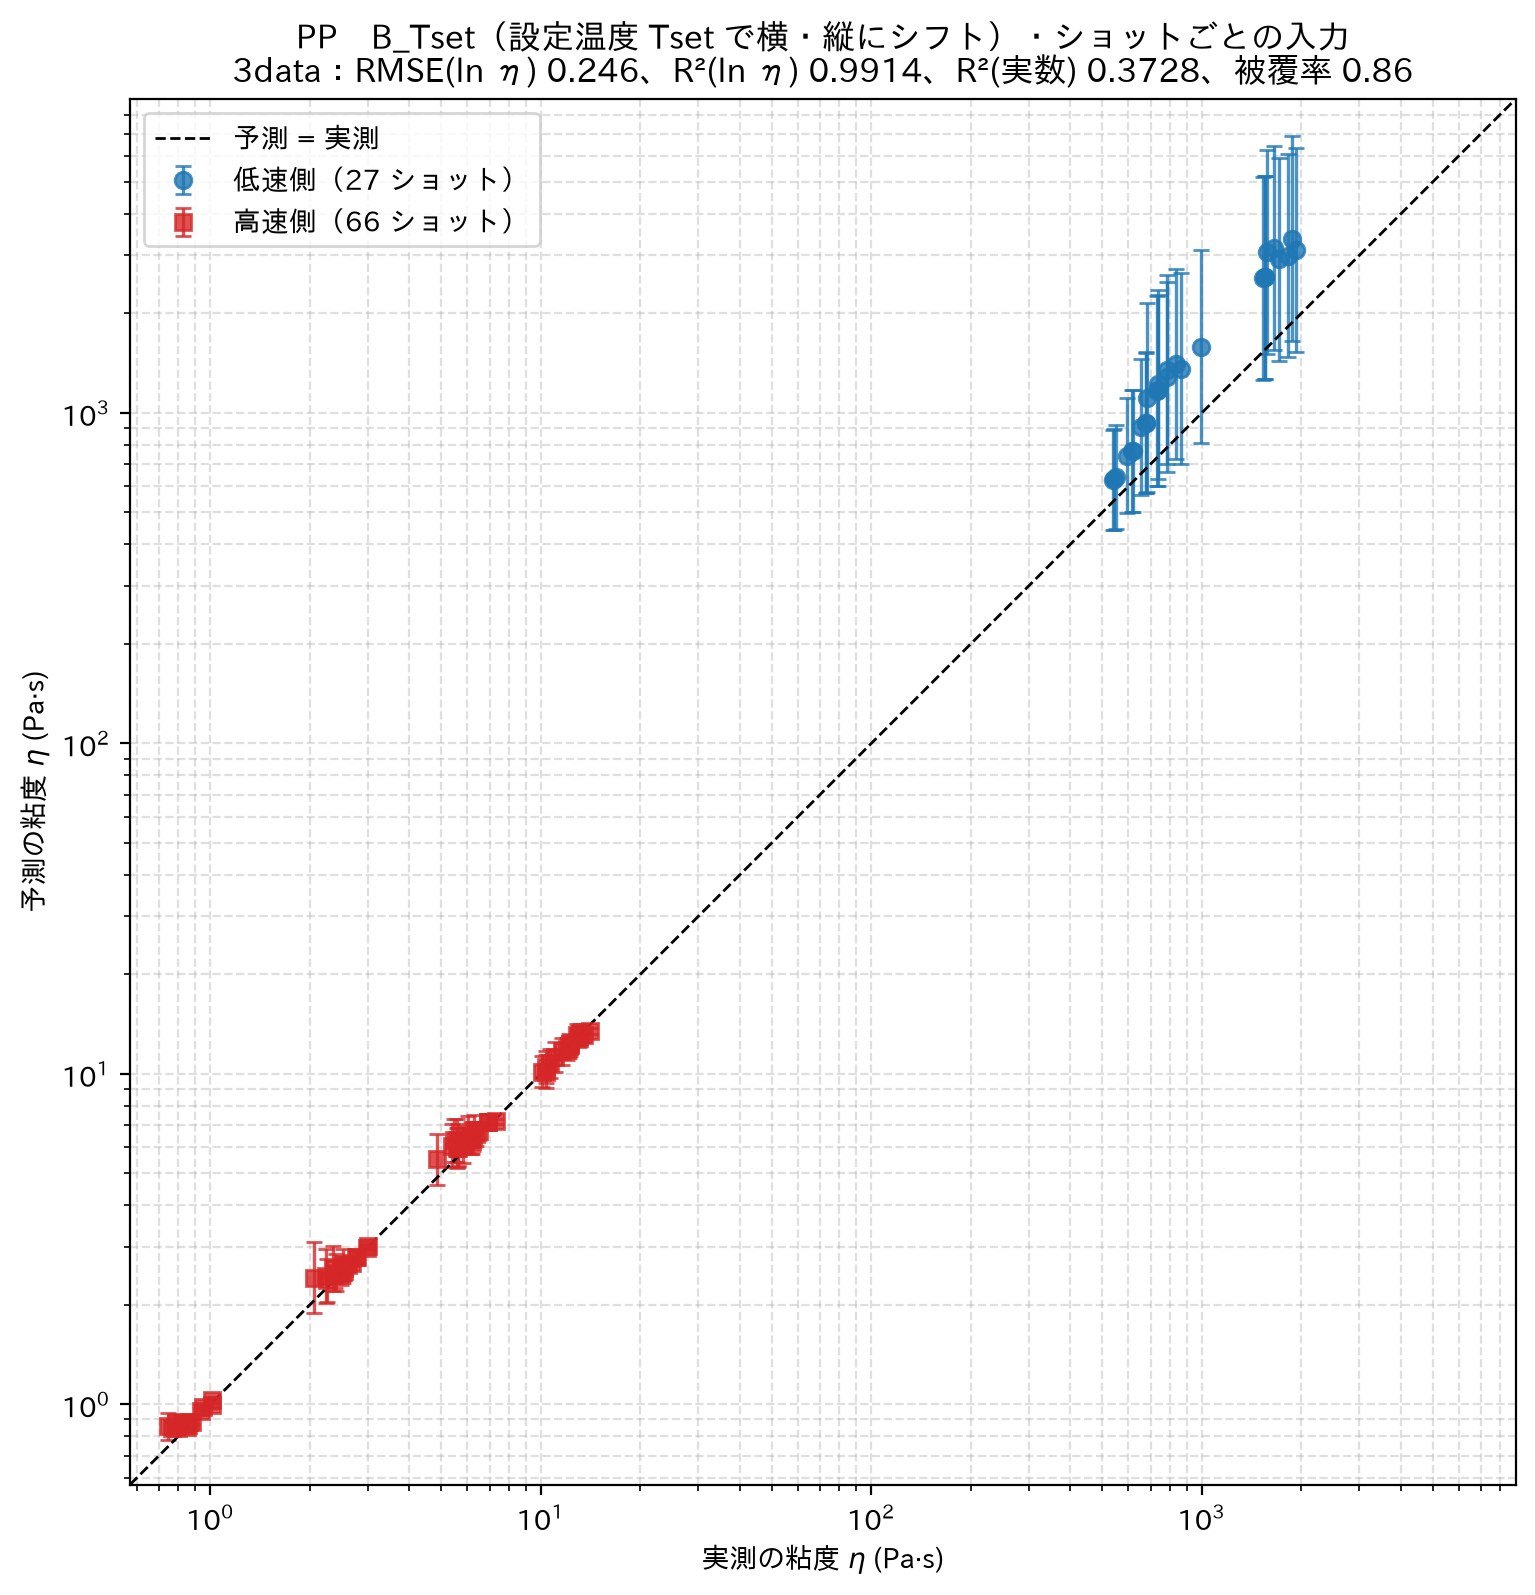
\includegraphics[width=0.7\linewidth]{01_バージンPP再々実験/01_バージンPP再々実験_学習結果/ショットごとの入力/B_Tset/予測検証_3data_パリティ.png}
\caption{横軸が実測、縦軸が予測の粘度。縦線が 95\% 予測区間}
\end{figure}
\begin{points}
\pt{何を示す図か}学習していない 3data（射出速度の両端）を予測した結果です。6月のノートのセル10 と同じ図です（ファイル：\file{<入力>/<モデル>/予測検証_3data_パリティ.png}）。
\pt{軸と記号}両対数。青が低速側（3・5 mm/s）、赤が高速側（280・320 mm/s）。破線が「予測 = 実測」。
\pt{見るポイント}点が破線の近くにあるか。縦線が破線をまたぐか（予測区間に入っているか）。
\pt{今回の結果}ショットごとの入力の B\_Tset で、RMSE は 0.246、粘度の実数の $R^2$ は 0.373、95\% 予測区間に入る割合は 0.86 です。条件平均の入力では、それぞれ 0.063・0.988・0.91 です（5.2 節の表）。低速側（左上の青）が、予測で大きく外れます。
\end{points}

\subsection{図10：3data の予測誤差の比較（PP・ショットごとの入力）}
\begin{figure}[H]
\centering
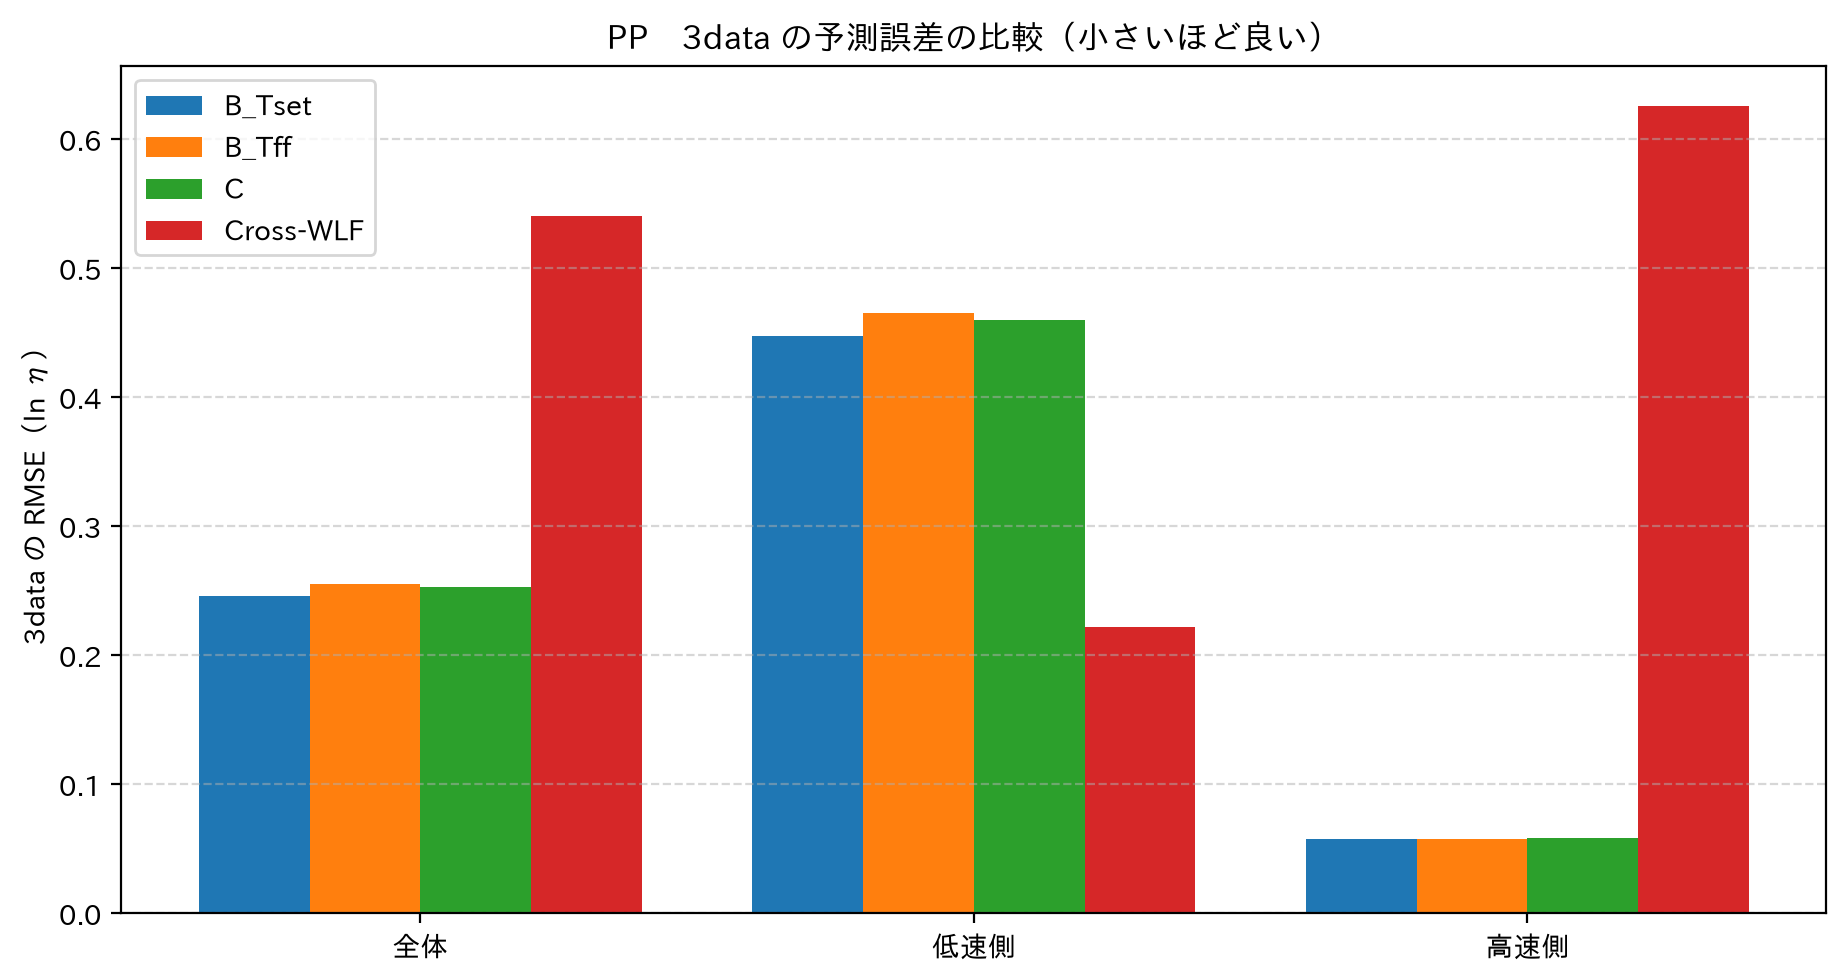
\includegraphics[width=0.8\linewidth]{01_バージンPP再々実験/01_バージンPP再々実験_学習結果/ショットごとの入力/比較/予測検証_RMSEの比較.png}
\caption{モデルごとの RMSE（全体・低速側・高速側）}
\end{figure}
\begin{points}
\pt{何を示す図か}全モデルと Cross-WLF の 3data の誤差を、範囲ごとに並べた図です（ファイル：\file{<入力>/比較/予測検証_RMSEの比較.png}）。
\pt{軸と記号}縦軸が RMSE（$\ln\eta$。小さいほどよい）。
\pt{見るポイント}シフトのあるモデル（B\_Tset・B\_Tff）が、基準の C と比べてどうか。
\pt{今回の結果}高速側（学習範囲の外の 280・320 mm/s）は、3 モデルとも同じくらい（0.057〜0.058）です。低速側（3・5 mm/s。外挿）は、3 モデルとも誤差が大きく（0.447〜0.465）、モデルの差は小さいです（5.2 節の表）。
\end{points}

\subsection{図11：乱数シードを変えて学習し直したときの、LML と 3data の RMSE（PP・条件平均の入力）}
\begin{figure}[H]
\centering
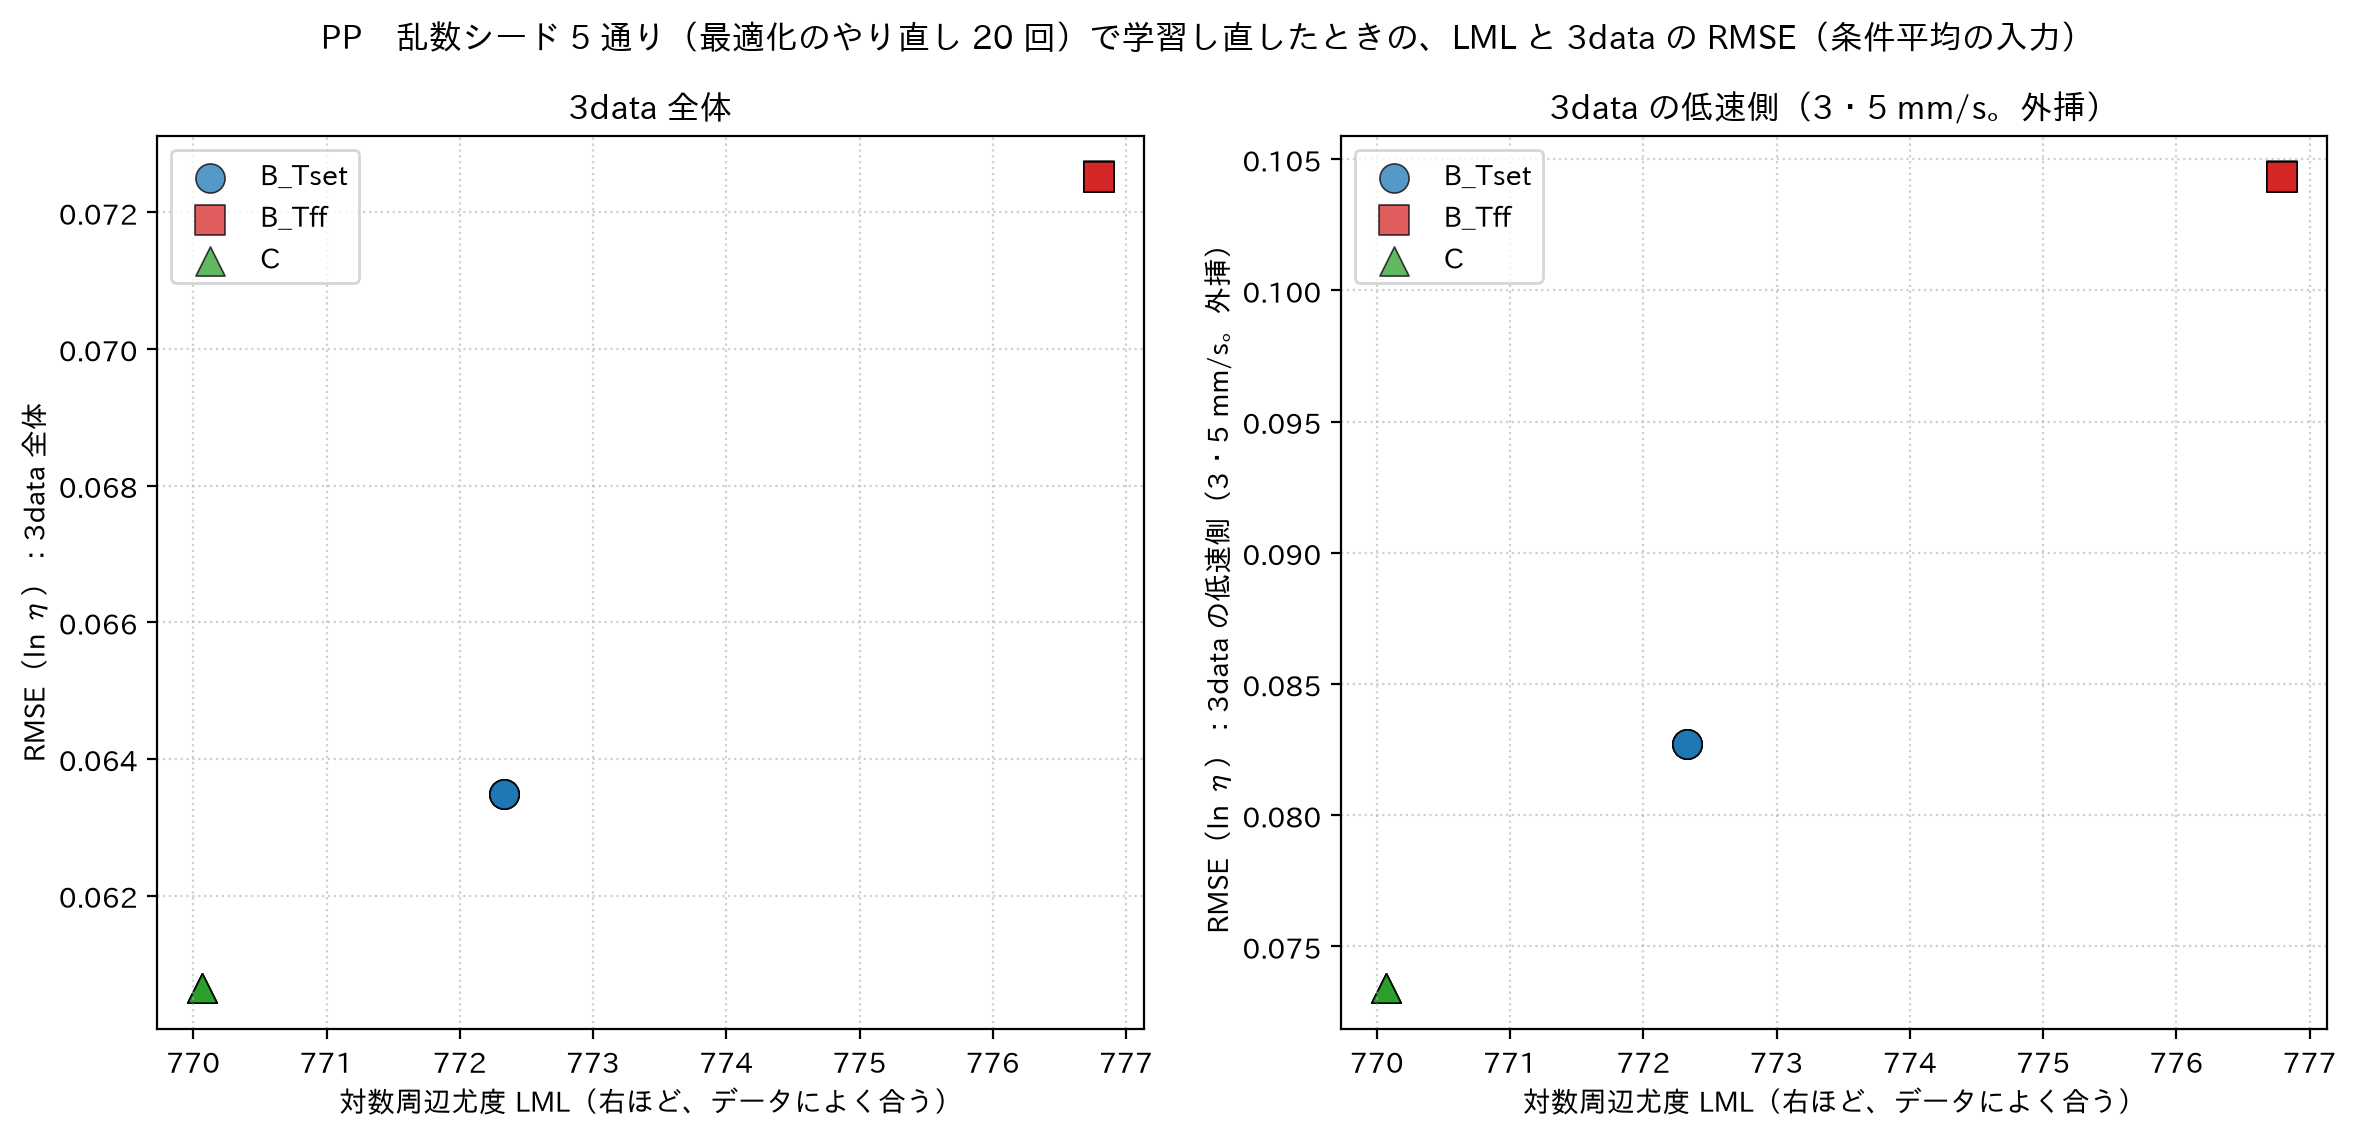
\includegraphics[width=1.0\linewidth]{01_バージンPP再々実験/01_バージンPP再々実験_学習結果/条件平均の入力/比較/乱数シードの確認.png}
\caption{点が 1 回の学習（乱数シード 5 通り、最適化のやり直し 20 回。係数 $\theta$ は固定）}
\end{figure}
\begin{points}
\pt{何を示す図か}最適化の初期値（乱数シード）を変えて、モデルを学習し直したときの、対数周辺尤度（LML）と 3data の RMSE の関係です（補助スクリプト \file{mat\_seed\_check.py}。ファイル：\file{<入力>/比較/乱数シードの確認.png}）。\textbf{条件平均の入力でだけ実施}しました（ショットごとの入力では未実施）。
\pt{軸と記号}横軸が LML（右ほど、データによく合う）、縦軸が RMSE（左：全体、右：低速側。小さいほどよい）。色と形がモデル。
\pt{見るポイント}同じモデルの点が、同じ LML・同じ RMSE に集まるか。LML がほぼ同じなのに、RMSE が大きく違う点があるか。
\pt{今回の結果}同じモデルでも、最適化が着く解によって、LML が 1 前後違うだけで、3data の（特に低速側の）RMSE が大きく変わる場合があります（5.5 節の表）。したがって、モデルどうしの 3data の RMSE の差は、この変動の範囲と比べて読む必要があります。
\end{points}

\subsection{図12：依存性グラフ（PP・B\_Tset・ショットごとの入力）}
\begin{figure}[H]
\centering
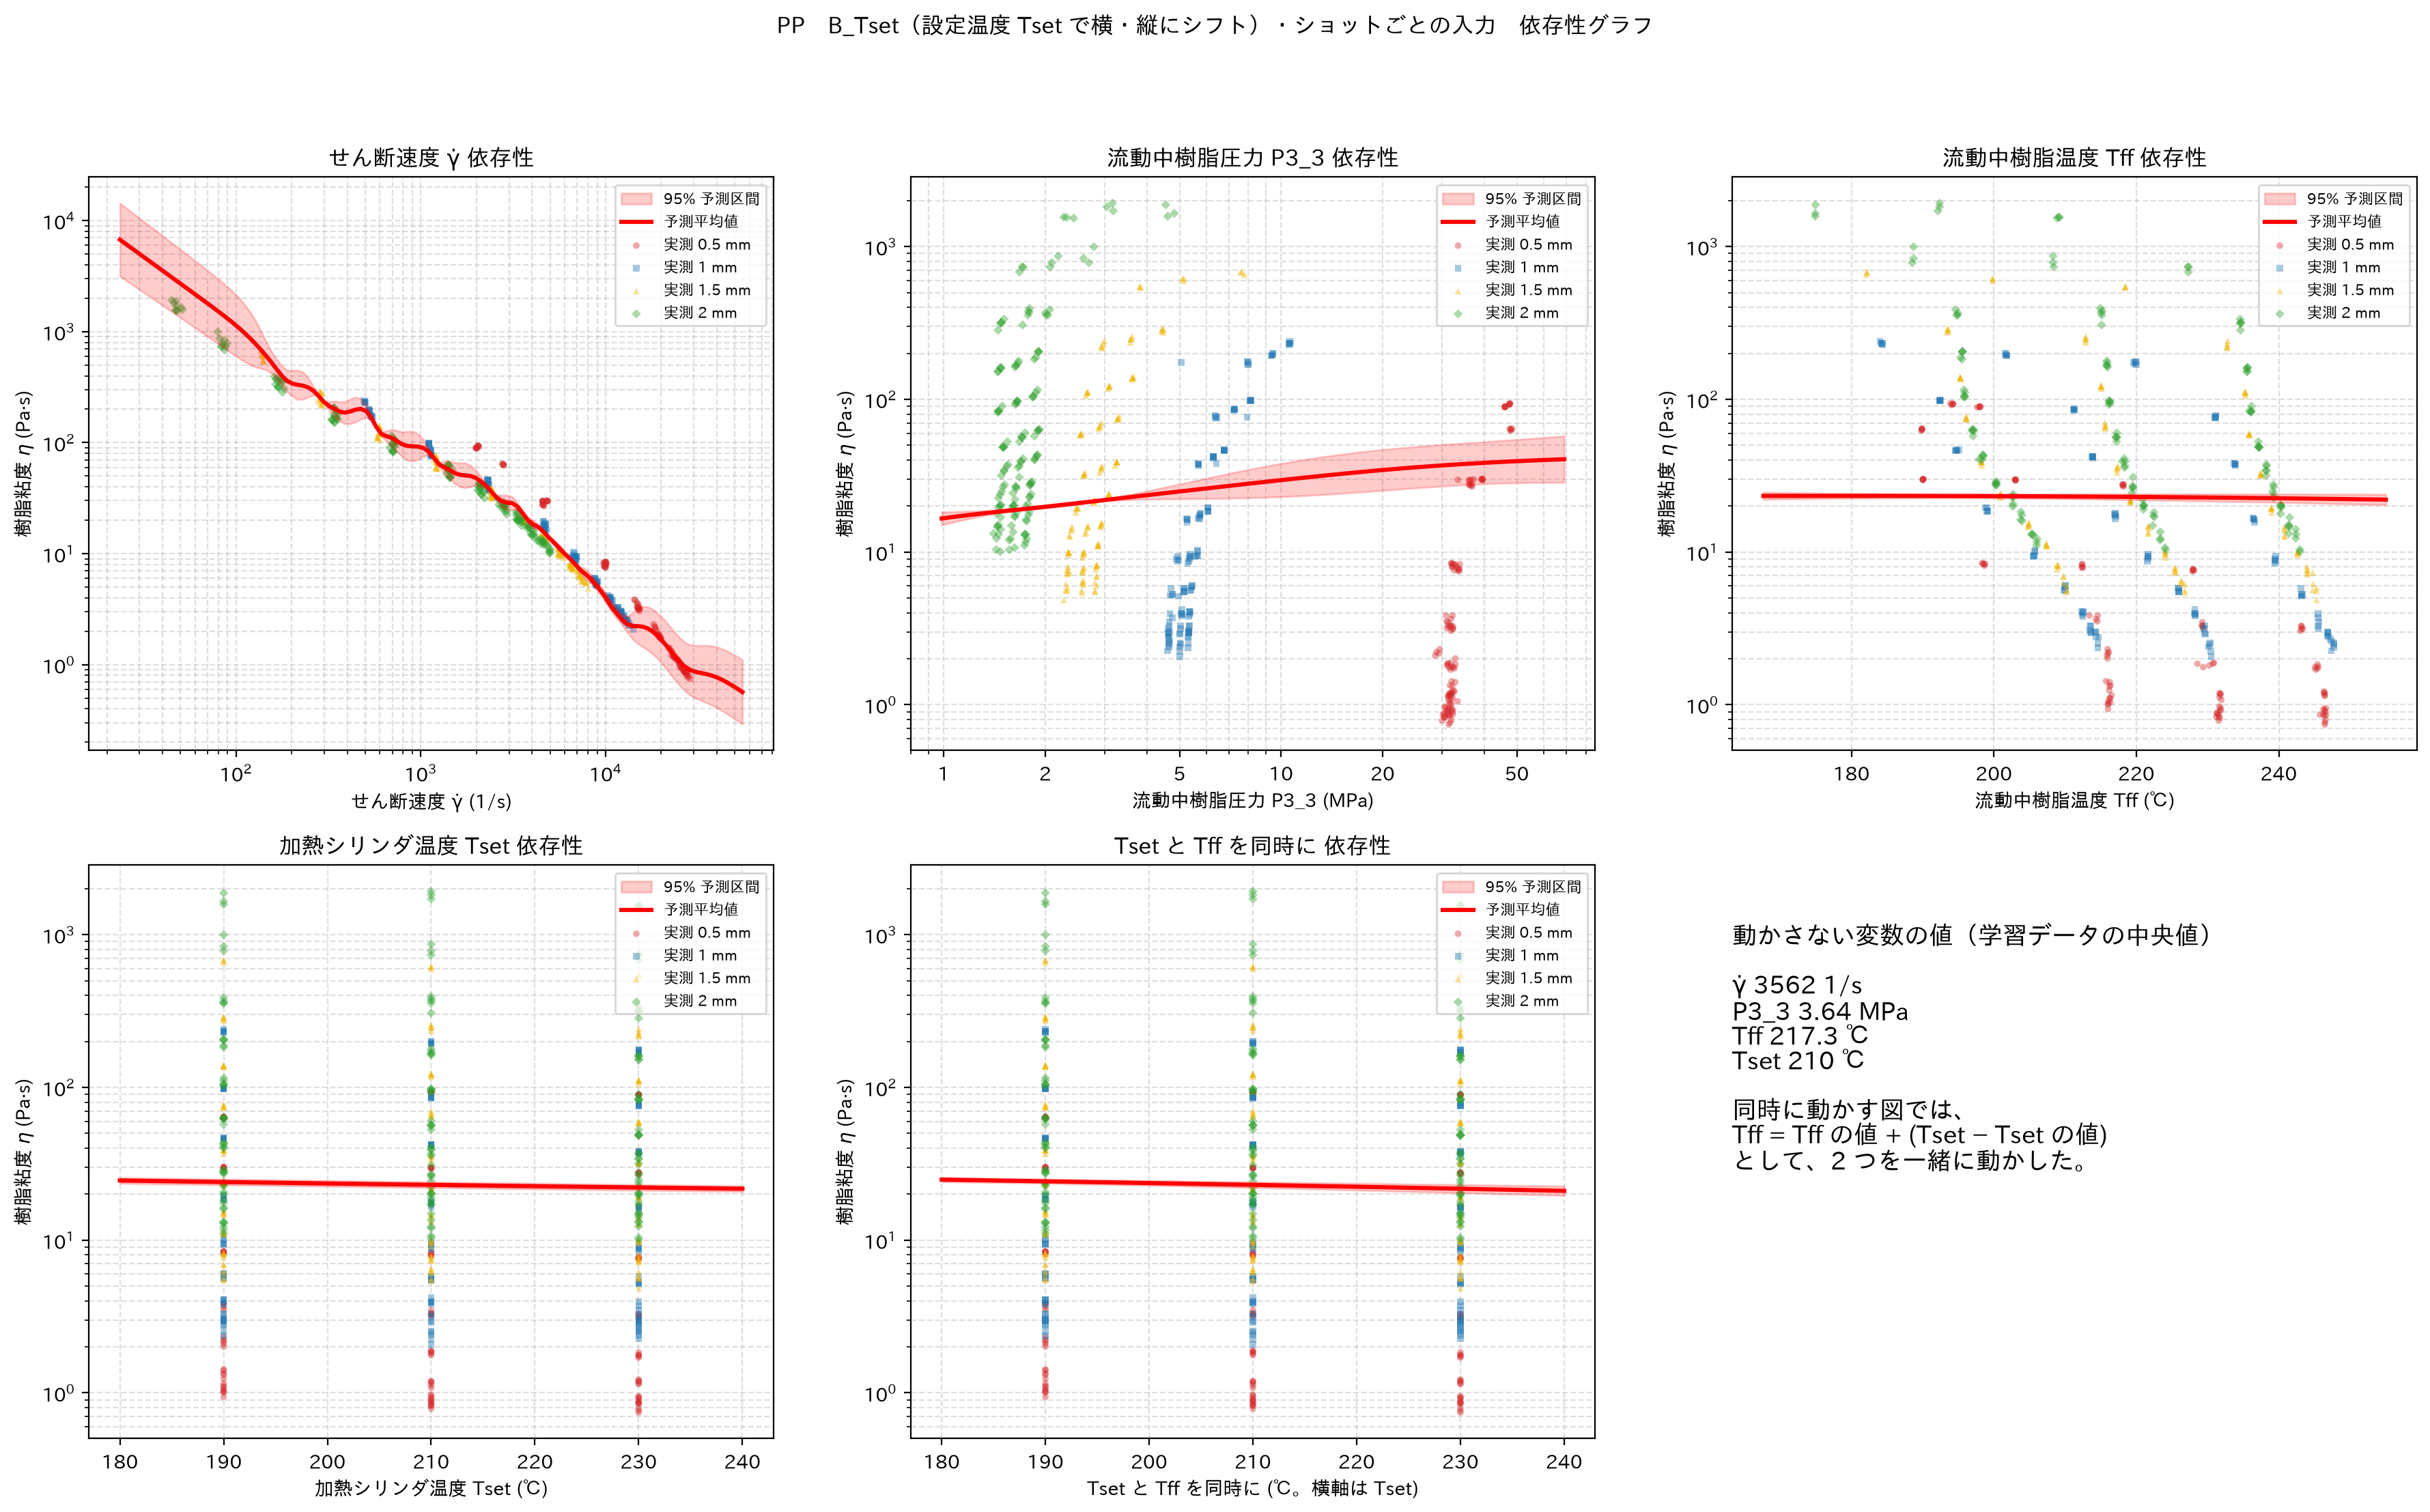
\includegraphics[width=1.0\linewidth]{01_バージンPP再々実験/01_バージンPP再々実験_学習結果/ショットごとの入力/B_Tset/依存性グラフ.png}
\caption{1 つの説明変数だけを動かしたときの予測（ほかは学習データの中央値、設定温度は $T_{\mathrm{ref}}$）}
\end{figure}
\begin{points}
\pt{何を示す図か}6月のノートのセル9 と同じ図です。各説明変数の効果の向きと大きさを見ます（ファイル：\file{<入力>/<モデル>/依存性グラフ.png}）。
\pt{軸と記号}縦軸は粘度（対数）。赤線が予測の平均、帯が 95\% 予測区間、点は実測（色は厚み）。右下から 2 番目の図は、$\Tset$ と $\Tff$ を同時に動かしたもの。
\pt{見るポイント}せん断速度を上げると粘度が下がるか、温度を上げると粘度が下がるか。
\pt{今回の結果}ほかの変数を固定しているので、実際には起こらない組み合わせも含みます。$\Tset$ だけ・$\Tff$ だけを動かすと、もう一方が固定のため、効果が小さく・逆向きに出ることがあります。$\Tset$ と $\Tff$ を同時に動かした図で、「温度を上げると粘度が下がる」ことを確かめます（ノートの判定）。
\end{points}

\subsection{図13：3次元グラフ（PP・B\_Tset・ショットごとの入力）}
\begin{figure}[H]
\centering
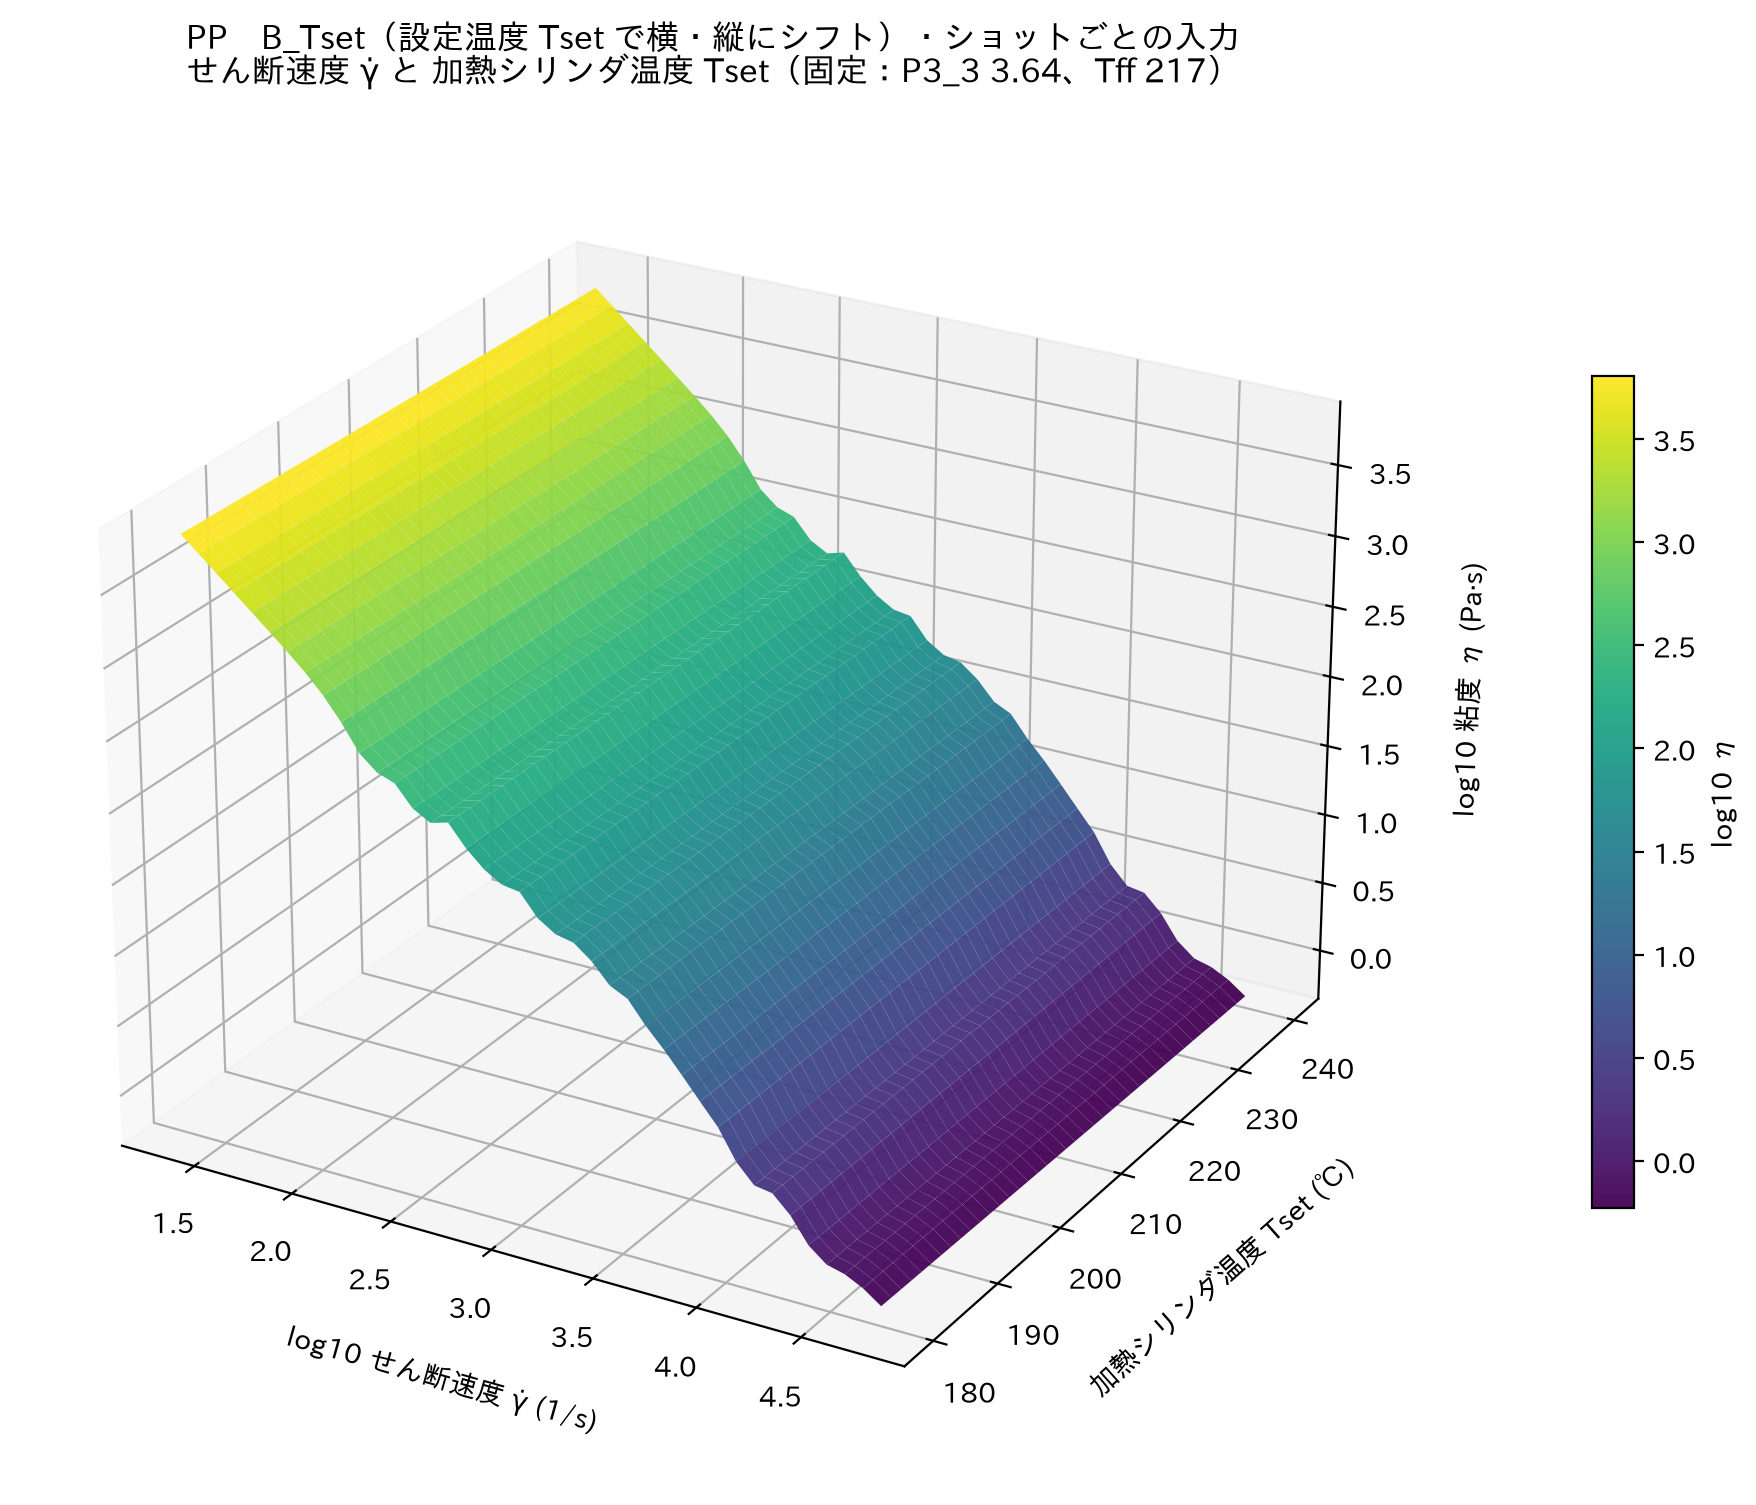
\includegraphics[width=0.75\linewidth]{01_バージンPP再々実験/01_バージンPP再々実験_学習結果/ショットごとの入力/B_Tset/3次元グラフ/3次元_gd_Tset.png}
\caption{せん断速度と設定温度を動かしたときの予測の粘度}
\end{figure}
\begin{points}
\pt{何を示す図か}6月のノートのセル12〜15 と同じ図です（ファイル：\file{<入力>/<モデル>/3次元グラフ/}。せん断速度と、設定温度・\PIII・$\Tff$ の組み合わせの 3 枚）。
\pt{軸と記号}横の 2 軸が動かした変数（せん断速度は常用対数）、縦軸が粘度の常用対数。
\pt{見るポイント}温度の向きの傾きが、どれくらいあるか。
\pt{今回の結果}依存性グラフと同じく、ほかの変数は固定です。
\end{points}

\subsection{図14：Cross-WLF との比較（PP・ショットごとの入力）}
\begin{figure}[H]
\centering
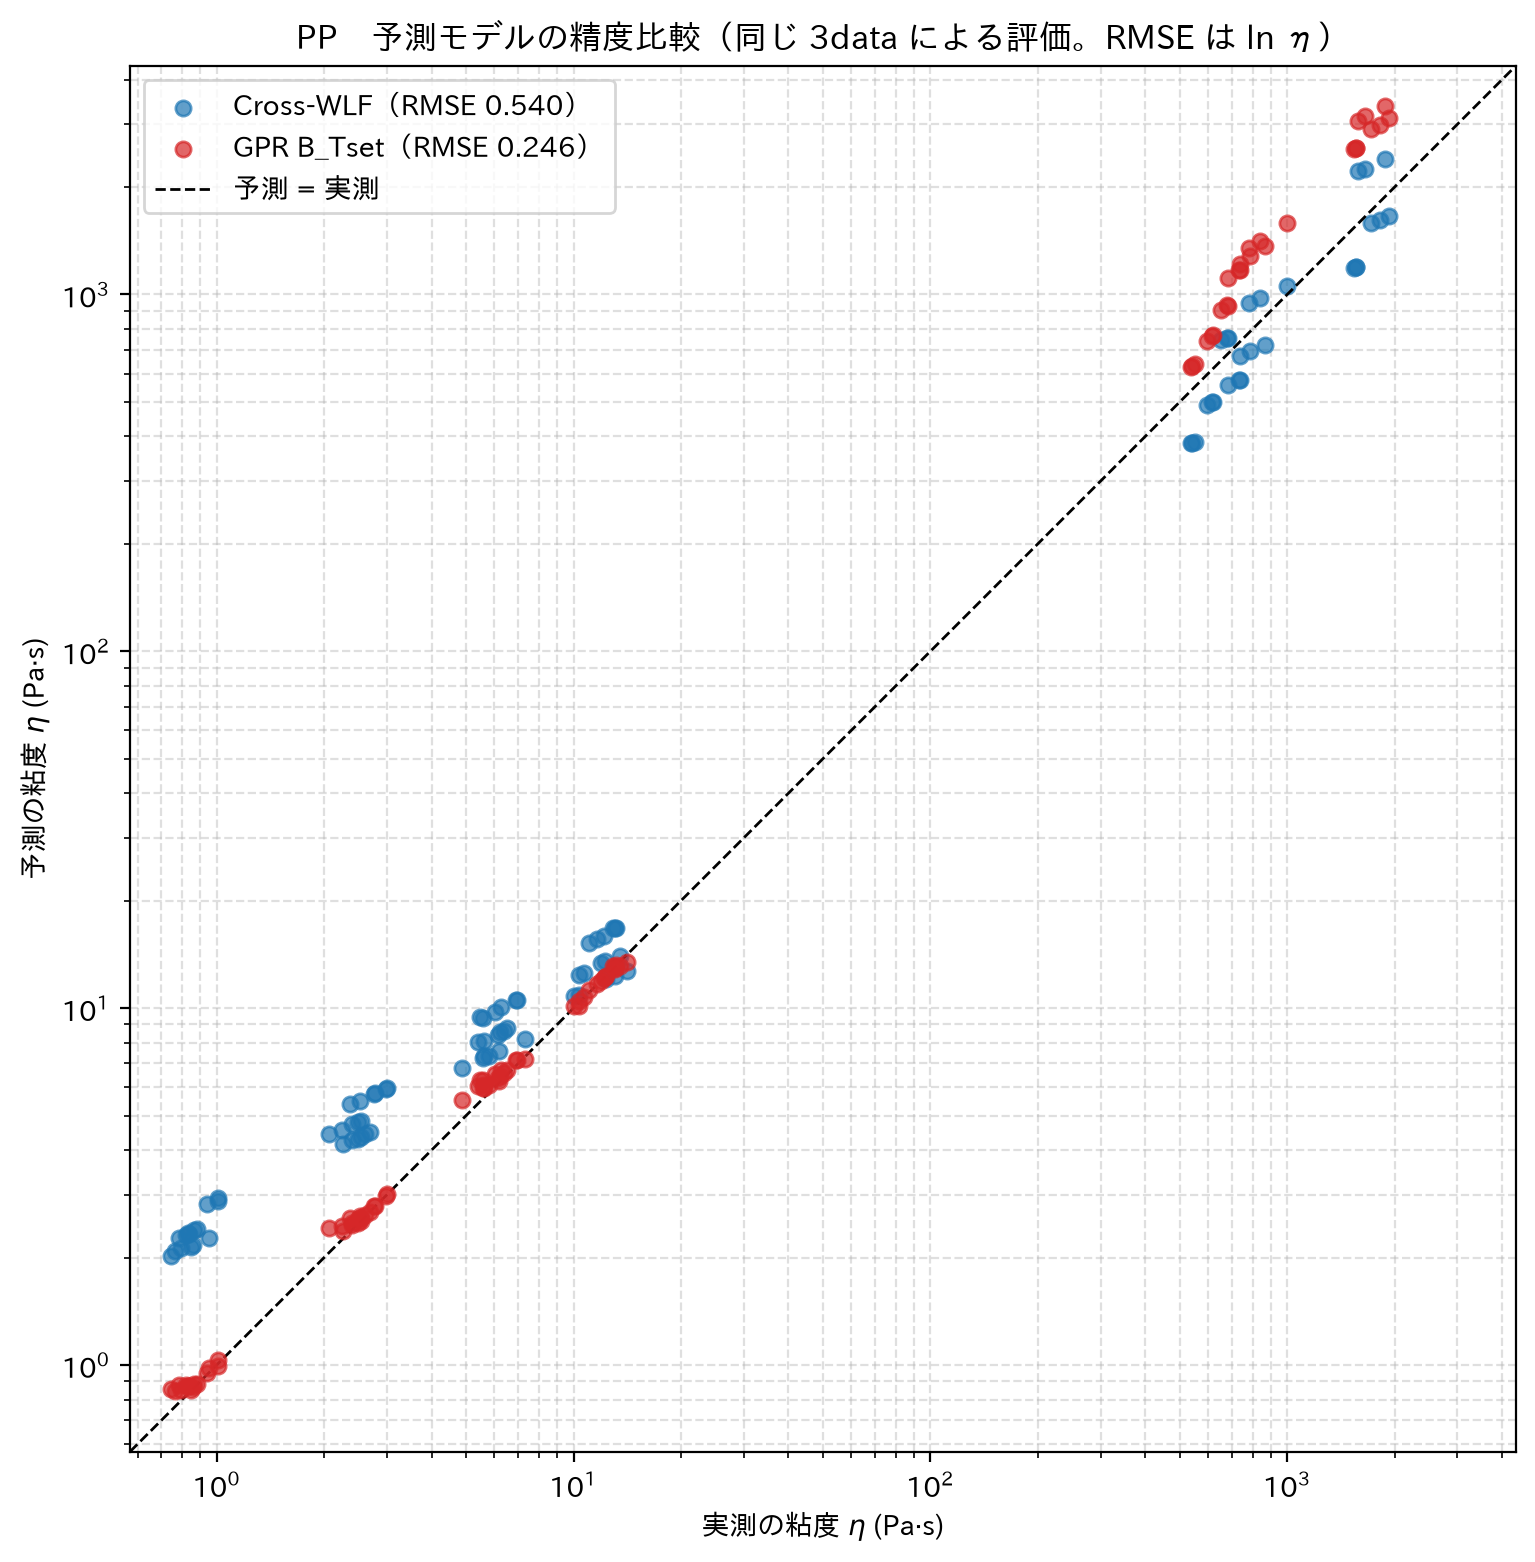
\includegraphics[width=0.7\linewidth]{01_バージンPP再々実験/01_バージンPP再々実験_学習結果/ショットごとの入力/比較/CrossWLFとの比較_パリティ.png}
\caption{同じ 3data での、Cross-WLF（青）と GPR（赤）の予測}
\end{figure}
\begin{points}
\pt{何を示す図か}6月のノートのセル11 と同じ比較です（ファイル：\file{<入力>/比較/CrossWLFとの比較_パリティ.png}）。
\pt{軸と記号}横軸が実測、縦軸が予測の粘度（両対数）。
\pt{見るポイント}どちらが破線に近いか。
\pt{今回の結果}Cross-WLF の RMSE は 0.540 で、GPR（B\_Tset、0.246）より大きい誤差です。Cross-WLF は、温度とせん断速度だけの式で、厚みの違い（\PIII\ に入る）を表せません。初期値を 12 通り変えても、係数は探索範囲の端に着き、同じ結果でした。あくまで参考です。
\end{points}

\subsection{図15：GPPS のシフトファクター（WLF 型。ショットごとの入力）}
\begin{figure}[H]
\centering
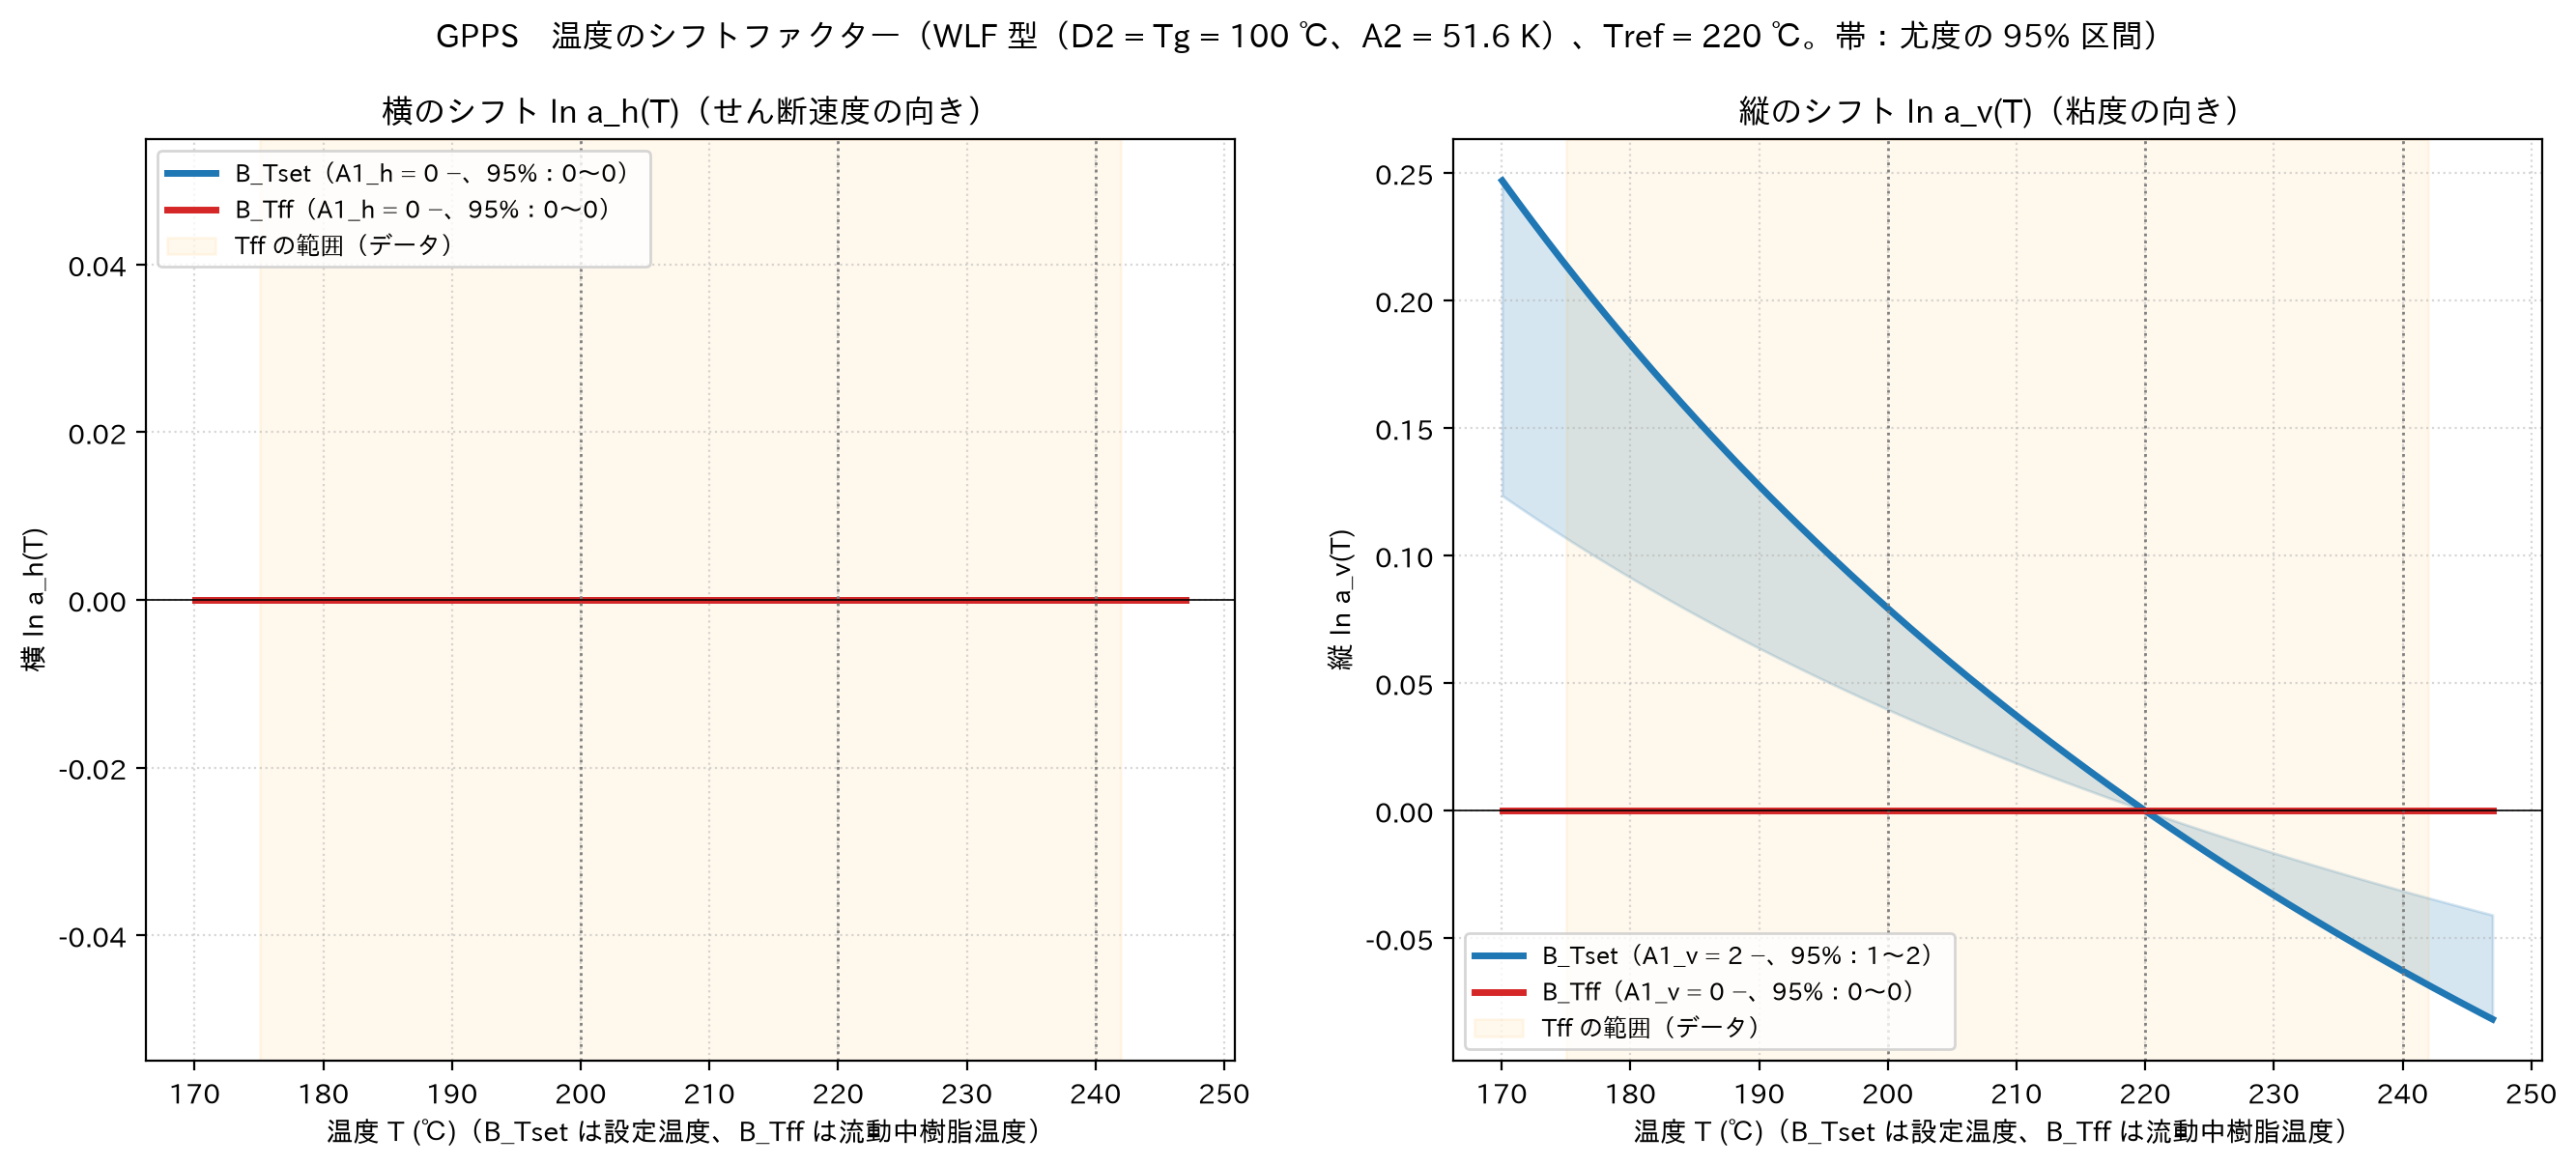
\includegraphics[width=0.9\linewidth]{03_GPPS実験/03_GPPS実験_学習結果/ショットごとの入力/比較/シフトファクター.png}
\caption{GPPS の $\ln a_h(T)$（左）と $\ln a_v(T)$（右）}
\end{figure}
\begin{points}
\pt{何を示す図か}非晶性の GPPS は、WLF 型でシフトファクターを表しました（$A_2=51.6$ K、$D_2=T_g$〔仮置き 100 ℃〕固定）。
\pt{軸と記号}図4と同じ。係数は $A_{1,h}$・$A_{1,v}$。
\pt{見るポイント}図4と同じ。
\pt{今回の結果}B\_Tset は $A_{1,h}=0$、$A_{1,v}=2$（$\Delta$LML 16.0）、B\_Tff は $A_{1,h}=0$、$A_{1,v}=0$（$\Delta$LML 0.0）でした。$T_g$ は仮置きなので、実際の値が分かれば、設定 \file{SHIFT_CFG} で直して実行し直します。
\end{points}

\subsection{図16：特徴スケール（PP・B\_Tset・ショットごとの入力）}
\begin{figure}[H]
\centering
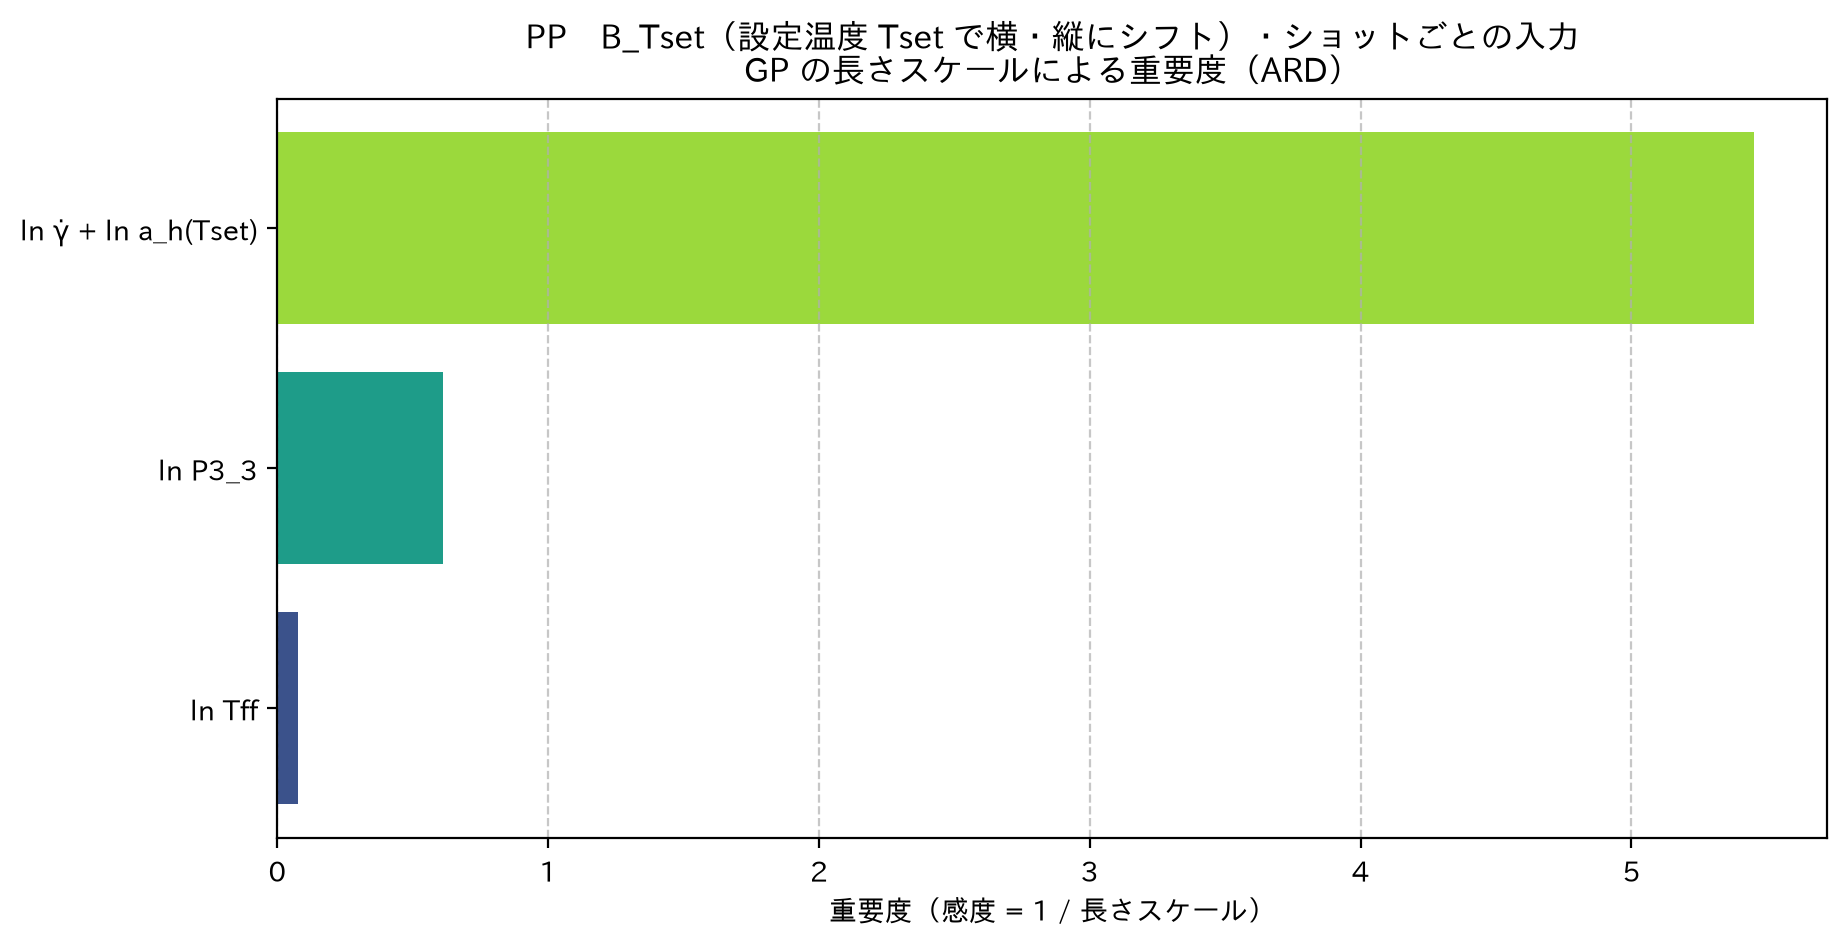
\includegraphics[width=0.7\linewidth]{01_バージンPP再々実験/01_バージンPP再々実験_学習結果/ショットごとの入力/B_Tset/特徴スケール.png}
\caption{特徴スケール（重要度 = 1／長さスケール）。損失関数の推移とカーネル行列は、同じフォルダの \file{損失関数の推移.png}・\file{カーネル行列.png}}
\end{figure}
\begin{points}
\pt{何を示す図か}6月のノートのセル7・7.5・8 と同じ図です。学習がうまく進んだか、どの入力に粘度が敏感かを見ます。
\pt{軸と記号}棒の長さが重要度（大きいほど、その入力の変化に粘度が敏感）。
\pt{見るポイント}どの入力の重要度が大きいか。シフトのあるモデルでは、シフトに使った温度の効果は係数 $\theta$ が担うので、ここには出ない。
\pt{今回の結果}ショットごとの入力では、換算せん断速度の重要度が、ほかの入力よりずっと大きくなります（長さスケールが短い）。5.3 節の表に、全モデルのハイパーパラメータをまとめました。
\end{points}


% =====================================================================
\section{表の見方}


\subsection{シフトファクターの推定}
\begin{table}[H]
\caption{最良の係数（括弧：おおよその 95\% 区間）、差 $\theta_v-\theta_h$、念入りに最適化した LML の、$\theta=0$ との差 $\Delta$LML、重ね合わせの残差（シフト前→後）。係数は、PP・粉砕材混合 PP が $\Eh$・$\Ev$（kJ/mol）、GPPS が $A_{1,h}$・$A_{1,v}$}\label{tab:shift}
\scriptsize
\begin{tabularx}{\linewidth}{@{}lllXXXrl@{}}
\toprule
入力 & 材料 & モデル & 横 $\theta_h$ & 縦 $\theta_v$ & 差 & $\Delta$LML & 重ね合わせ \\
\midrule
ショットごとの入力 & PP & B\_Tset & 0（0〜0） & 4（1〜6） & 4（1〜6） & 3.2 & 0.067→0.043 \\
 &  & B\_Tff & 0（0〜0） & 4（0〜8） & 4（0〜8） & 1.1 & 0.067→0.044 \\
 & 粉砕材混合 PP & B\_Tset & 0（-1〜0） & 6（2〜8） & 6（3〜8） & 9.6 & 0.070→0.042 \\
 &  & B\_Tff & 0（-1〜0） & -1（-5〜1） & -1（-4〜1） & 0.3 & 0.070→0.076 \\
 & GPPS & B\_Tset & 0（0〜0） & 2（1〜2） & 2（1〜2） & 16.0 & 0.121→0.075 \\
 &  & B\_Tff & 0（0〜0） & 0（0〜0） & 0（0〜0） & 0.0 & 0.121→0.121 \\
\midrule
条件平均の入力 & PP & B\_Tset & 9（5〜10） & 14（5〜18） & 5（0〜9） & 1.5 & 0.067→0.067 \\
 &  & B\_Tff & 8（5〜13） & 20（15〜29） & 12（8〜17） & 8.3 & 0.067→0.030 \\
 & 粉砕材混合 PP & B\_Tset & 3（-1〜7） & 0（-5〜5） & -3（-7〜1） & 1.7 & 0.070→0.103 \\
 &  & B\_Tff & 6（2〜10） & 17（11〜25） & 11（6〜15） & 4.5 & 0.070→0.036 \\
 & GPPS & B\_Tset & 3（2〜3） & 6（3〜7） & 3（1〜4） & 3.2 & 0.121→0.086 \\
 &  & B\_Tff & 3（1〜4） & 8（6〜12） & 5（3〜8） & 10.7 & 0.121→0.048 \\

\bottomrule
\end{tabularx}
\end{table}
\begin{points}
\pt{読み方}$\Delta$LML が 3.0 以上なら、その温度をシフトの形で入れる効果が、尤度比検定の 5\% 基準で認められます。小さければ、シフトなし（その温度を使わない）でも、ほとんど同じくらいデータに合います。尾根があるので、個々の係数の区間は、計算した範囲に左右されます。差 $\theta_v-\theta_h$ が、最もよく決まる量です。ショットごとの入力（既定）では、$\theta_h$ はほぼすべて 0 で、B\_Tset の縦のシフトだけが支持されました。ショットごとの尤度は、設定温度の目印が入力に入る影響も受けます（本体の手順5a の注意）。条件平均の入力（参考）では、B\_Tff が支持されました。
\end{points}

\subsection{3data の予測検証}
\begin{table}[H]
\caption{3data の RMSE（$\ln\eta$）、95\% 予測区間に入る割合（被覆率）、粘度の実数の $R^2$（6月のノートと同じ）}\label{tab:met}
\scriptsize
\begin{tabularx}{\linewidth}{@{}lllrrrrr@{}}
\toprule
入力 & 材料 & モデル & 全体 & 低速側 & 高速側 & 被覆率 & $R^2$（実数） \\
\midrule
ショットごとの入力 & PP & B\_Tset & 0.246 & 0.447 & 0.057 & 0.86 & 0.373 \\
 &  & B\_Tff & 0.255 & 0.465 & 0.057 & 0.87 & 0.307 \\
 &  & C & 0.252 & 0.460 & 0.058 & 0.86 & 0.332 \\
 &  & Cross-WLF & 0.540 & 0.222 & 0.625 & 0.81 & 0.931 \\
\midrule
 & 粉砕材混合 PP & B\_Tset & 0.193 & 0.331 & 0.048 & 0.92 & 0.697 \\
 &  & B\_Tff & 0.193 & 0.335 & 0.035 & 0.91 & 0.697 \\
 &  & C & 0.184 & 0.316 & 0.043 & 0.92 & 0.738 \\
 &  & Cross-WLF & 0.467 & 0.201 & 0.551 & 0.83 & 0.934 \\
\midrule
 & GPPS & B\_Tset & 0.114 & 0.166 & 0.063 & 0.82 & 0.970 \\
 &  & B\_Tff & 0.131 & 0.194 & 0.065 & 0.82 & 0.961 \\
 &  & C & 0.129 & 0.189 & 0.066 & 0.84 & 0.962 \\
 &  & Cross-WLF & 0.676 & 0.736 & 0.635 & 0.59 & 0.541 \\
\midrule
条件平均の入力 & PP & B\_Tset & 0.063 & 0.083 & 0.054 & 0.91 & 0.988 \\
 &  & B\_Tff & 0.123 & 0.213 & 0.054 & 0.89 & 0.848 \\
 &  & C & 0.061 & 0.073 & 0.055 & 0.90 & 0.991 \\
 &  & Cross-WLF & 0.540 & 0.222 & 0.625 & 0.81 & 0.931 \\
\midrule
 & 粉砕材混合 PP & B\_Tset & 0.096 & 0.157 & 0.040 & 0.98 & 0.931 \\
 &  & B\_Tff & 0.047 & 0.059 & 0.040 & 0.98 & 0.994 \\
 &  & C & 0.075 & 0.119 & 0.039 & 0.98 & 0.973 \\
 &  & Cross-WLF & 0.467 & 0.201 & 0.551 & 0.83 & 0.934 \\
\midrule
 & GPPS & B\_Tset & 0.151 & 0.230 & 0.064 & 0.86 & 0.928 \\
 &  & B\_Tff & 0.090 & 0.121 & 0.064 & 0.93 & 0.980 \\
 &  & C & 0.112 & 0.161 & 0.064 & 0.94 & 0.946 \\
 &  & Cross-WLF & 0.676 & 0.736 & 0.635 & 0.59 & 0.541 \\

\bottomrule
\end{tabularx}
\end{table}
\begin{points}
\pt{読み方}RMSE は小さいほどよい（0.1 は粘度で約 10\%）。被覆率は 0.95 に近いほどよい。$R^2$（実数）は、粘度の大きい低速側の誤差に強く左右されます。Cross-WLF は、6月のノートと同じく温度に $\Tff$ を使い、一部の係数を固定して 5data に当てはめたもの（5.4 節）。\textbf{ショットごとの入力は、低速側の誤差が大きい}（条件平均の 2〜5 倍）です。
\end{points}

\subsection{ハイパーパラメータ（ショットごとの入力）}
\begin{table}[H]
\caption{最終モデルのハイパーパラメータ（振幅は $\sqrt{\text{振幅}^2}$、長さスケールは標準化した入力に対する値）}\label{tab:hp}
\scriptsize
\begin{tabularx}{\linewidth}{@{}llrrrrX@{}}
\toprule
材料 & モデル & LML & 振幅 & 線形項の振幅 & ノイズ $\sigma_n$ & 長さスケール \\
\midrule
PP & B\_Tset & 1273.5 & 0.289 & 0.913 & 0.007 & ln γ̇ + ln a\_h(Tset) 0.183、ln P3\_3 1.64、ln Tff 13.3 \\
 & B\_Tff & 1275.3 & 0.281 & 0.907 & 0.007 & ln P3\_3 1.61、ln γ̇ + ln a\_h(Tff) 0.18、Tset 15.5 \\
 & C & 1271.4 & 0.285 & 0.786 & 0.007 & ln P3\_3 1.61、ln Tff 37、Tset 16.7、ln γ̇ 0.181 \\
\midrule
粉砕材混合 PP & B\_Tset & 1324.5 & 0.333 & 0.885 & 0.006 & ln γ̇ + ln a\_h(Tset) 0.22、ln P3\_3 1.58、ln Tff 15.3 \\
 & B\_Tff & 1323.4 & 0.337 & 0.871 & 0.006 & ln P3\_3 1.66、ln γ̇ + ln a\_h(Tff) 0.213、Tset 20.1 \\
 & C & 1322.2 & 0.336 & 0.751 & 0.006 & ln P3\_3 1.61、ln Tff 16.7、Tset 100、ln γ̇ 0.22 \\
\midrule
GPPS & B\_Tset & 929.6 & 0.242 & 0.812 & 0.007 & ln γ̇ + ln a\_h(Tset) 0.218、ln P3\_3 3.37、ln Tff 10.9 \\
 & B\_Tff & 929.1 & 0.253 & 0.815 & 0.007 & ln P3\_3 3.28、ln γ̇ + ln a\_h(Tff) 0.22、Tset 12.9 \\
 & C & 929.8 & 0.265 & 0.704 & 0.007 & ln P3\_3 3.41、ln Tff 13.8、Tset 31.5、ln γ̇ 0.229 \\

\bottomrule
\end{tabularx}
\end{table}
\begin{points}
\pt{読み方}ノイズの標準偏差（約 0.006〜0.007）は、同じ条件のショット間のばらつき（約 0.04〜0.05）よりずっと小さく出ます。ショットごとの $\gd$ が、同じ条件の中の粘度のゆれの大部分を説明するためです（条件平均の入力では、ノイズの標準偏差がショット間のばらつきとほぼ同じ）。長さスケールが 100（上限）に届いた入力は、粘度にほとんど効いていない（線形項が担う）入力です。振幅と線形項の振幅は、本体の手順5b の MCMC でも、データでは決まりにくいことが分かっています。
\end{points}

\subsection{Cross-WLF の係数（ショットごとの入力のノートで当てはめたもの）}
\begin{table}[H]
\caption{Cross-WLF の係数（$D_3=0$。$D_2$ は K。「範囲の端」は、探索の範囲の端に届いた係数）}\label{tab:cw}
\scriptsize
\begin{tabularx}{\linewidth}{@{}lX@{}}
\toprule
材料 & 係数 \\
\midrule
PP & n = 0.05588（探索）、tau\_star = 3137（探索）、D1 = 9.997e+29（探索）、D2 = 450（探索（範囲の端））、A1 = 30.9（固定）、A2 = 43.45（固定） \\
粉砕材混合 PP & n = 0.05281（探索）、tau\_star = 3599（探索）、D1 = 9.581e+29（探索）、D2 = 450（探索（範囲の端））、A1 = 30.9（固定）、A2 = 43.45（固定） \\
GPPS & n = 0.04185（探索）、tau\_star = 4.869e+04（探索）、D1 = 1e+30（探索（範囲の端））、D2 = 373.1（固定）、A1 = 80（探索（範囲の端））、A2 = 51.6（固定） \\
\bottomrule
\end{tabularx}
\end{table}

\subsection{乱数シードの確認（条件平均の入力）}
\begin{table}[H]
\caption{乱数シード 5 通り（最適化のやり直し 20 回。係数 $\theta$ は固定）で学習し直したときの、LML と 3data の RMSE の範囲。右端は、ノートの最終モデルの値（括弧：低速側）}\label{tab:seed}
\scriptsize
\begin{tabularx}{\linewidth}{@{}llXXXX@{}}
\toprule
材料 & モデル & LML & RMSE 全体 & RMSE 低速側 & ノートの最終モデル \\
\midrule
PP & B\_Tset & 772.3〜772.3 & 0.063〜0.063 & 0.083〜0.083 & 0.063（0.083） \\
 & B\_Tff & 776.8〜776.8 & 0.073〜0.073 & 0.104〜0.104 & 0.123（0.213） \\
 & C & 770.1〜770.1 & 0.061〜0.061 & 0.073〜0.073 & 0.061（0.073） \\
\midrule
粉砕材混合 PP & B\_Tset & 771.8〜771.8 & 0.073〜0.073 & 0.113〜0.113 & 0.096（0.157） \\
 & B\_Tff & 774.5〜774.7 & 0.047〜0.114 & 0.059〜0.191 & 0.047（0.059） \\
 & C & 770.7〜770.7 & 0.075〜0.075 & 0.119〜0.119 & 0.075（0.119） \\
\midrule
GPPS & B\_Tset & 492.2〜492.2 & 0.151〜0.151 & 0.230〜0.230 & 0.151（0.230） \\
 & B\_Tff & 496.2〜496.2 & 0.090〜0.090 & 0.121〜0.121 & 0.090（0.121） \\
 & C & 487.7〜488.1 & 0.063〜0.112 & 0.060〜0.161 & 0.112（0.161） \\

\bottomrule
\end{tabularx}
\end{table}
\begin{points}
\pt{読み方}LML の範囲が狭く、RMSE の範囲も狭ければ、最適化は安定しています。LML の範囲が 1 前後でも RMSE の範囲が広ければ、「LML がほぼ同じ解が複数あり、予測（特に外挿）が違う」ことを表します。
\end{points}


% =====================================================================
\section{結論と、これからの選択肢}


ノートの判定は、OK ショットごとの入力で 68・条件平均の入力で 67 個、★ それぞれ 7・8 個でした。以下、主にショットごとの入力（既定）の結果をまとめ、条件平均の入力（参考）と比べます。

\begin{enumerate}[itemsep=0.8ex,topsep=0.6ex]
\item \textbf{プログラムと結果}：6月のノートを基準に、材料ごとのデータ（5data で学習、3data で検証）を一人で実行できるノートを作りました。結果は、各材料フォルダの \file{<材料フォルダ>_学習結果/<入力の取り方>/} にあります。ノートは 3 材料 $\times$ 3 モデルを学習し、ショットごとの入力で約 43 分（そのうち、大部分はプロファイル尤度）かかります。
\item \textbf{データと外れ値}：規則 f で拾ったのは、PP の P03 の 1 条件だけで、除外しました。GPPS の 3data には \PIII\ が負のショットがあり（P09）、除外しました。\PIII\ は、粘度の算出式の圧力ではありませんが、流れの結果として測られる量で、成形の前には分かりません。このモデルは、「測った流れの状態（$\gd$・\PIII・$\Tff$）と設定温度 $\rightarrow$ 粘度」のモデルです。
\item \textbf{入力の取り方（ユーザーの決定、10 月 23 日）}：ショットごとの値で学習する仕様にしました（既定 \file{"shot"}）。ショットごとの入力では、同じ条件の中のせん断速度と粘度のゆれ（センサへの到達時刻のゆれ）に GP が合わせるので、$\ln\gd$ の長さスケールが短く（C で 0.18・0.22・0.23。条件平均では 6.4・5.4・7.0）、ノイズの標準偏差も小さく出ます（0.007・0.006・0.007。条件平均では 0.039・0.038・0.049）。その結果、曲線がデータの範囲の中でも波打ち、3data の低速側の誤差が大きくなりました（C の RMSE：ショットごと 0.460・0.316・0.189、条件平均 0.073・0.119・0.161。PP・粉砕材混合 PP・GPPS）。
\item \textbf{温度のシフト}：ショットごとの入力では、\textbf{加熱シリンダ温度 $\Tset$ でずらす B\_Tset のシフトが支持され}（$\theta=0$ との LML の差：3.2・9.6・16.0。基準 3.0）、\textbf{流動中樹脂温度 $\Tff$ でずらす B\_Tff は支持されませんでした}（1.1・0.3・0.0）。B\_Tset の横の係数は 3 材料とも 0 で、縦のシフト（同じせん断速度での粘度の倍率）だけが支持されました。条件平均の入力では逆で、B\_Tff が支持され（8.3・4.5・10.7）、B\_Tset は基準に届かないか、ぎりぎりでした（1.5・1.7・3.2）。\textbf{どちらの温度がシフトに適するかは、入力の取り方に左右されます}。ショットごとの入力では、ショットごとに変わる $\Tff$ が GP の入力として粘度の違いを担うため、と考えられます。
\item \textbf{シフトの解釈の注意}：$\Tff$ は、せん断速度と連動して動きます（低速ほど低く、高速ほど高い。せん断発熱）。$\Tff$ でずらすシフトは、「設定温度の違い」だけでなく「見かけの粘度に含まれる、せん断発熱の効果」も拾いうるので、どちらの入力の取り方でも、温度の効果をシフトとして取り出すのは難しい面があります。総合グラフ（図8）は、\PIII\ と $\Tff$ を固定した断面で、シフトの証拠にはなりません。
\item \textbf{3data の予測}：高速側（280・320 mm/s の外挿）は、3 モデルともほぼ同じ精度です（RMSE 0.035〜0.066）。低速側（3・5 mm/s の外挿）は誤差が大きく、全体の RMSE が最小のモデルは、PP B\_Tset（0.246）、粉砕材混合 PP C（0.184）、GPPS B\_Tset（0.114）でした。条件平均の入力の最小（0.061・0.047・0.090）より大きい誤差です。乱数シードを変えた確認（5.5 節。条件平均の入力で実施）では、同じモデルでも全体の RMSE が最大で最小の 2.4 倍まで変わったので、モデルどうしの差は、この変動と比べて読む必要があります（ショットごとの入力では、まだ実施していません）。
\item \textbf{Cross-WLF との比較}：参考の Cross-WLF は、RMSE が 0.54（PP）・0.47（粉砕材混合 PP）・0.68（GPPS）で、GPR（0.11〜0.25）より大きい誤差です。厚みの違いを表せないためと考えられます。
\item \textbf{ノートの ★ の意味}：ショットごとの入力では、主に 5 尤度・6 シフト の節で、B\_Tff の $\Delta$LML が基準に届かない、縦のシフトの向きや重ね合わせの残差が期待どおりでない（B\_Tff の係数がほぼ 0 のため）、という注意が出ました。エラーではなく、結果を読むときの注意点です。
\end{enumerate}

\subsection{これからの選択肢（ユーザーの判断）}
\begin{enumerate}[itemsep=0.6ex,topsep=0.6ex]
\item \textbf{入力の取り方}：ノートの既定はショットごとです（10 月 23 日）。3data の予測誤差は、条件平均の入力のほうが小さくなりました。条件平均に戻すときは、設定 \file{INPUT_MODE} を \file{"cond"} にします（結果は \file{条件平均の入力/} に残っています）。
\item \textbf{乱数シードの確認}：ショットごとの入力でも、\file{mat_seed_check.py shot} で、最適化の運による RMSE の変動を確かめられます（未実施）。
\item \textbf{P09 の扱い}：GPPS の 3data、200 ℃・1.5 mm・3 mm/s は、残るショット 001 も疑わしいので、条件全体を除くか決めてください（一覧の「ショット」列を空欄にします）。
\item \textbf{GPPS の $T_g$}：仮置きの 100 ℃ です。実際の値が分かれば、\file{SHIFT_CFG} で直して実行し直します。
\item \textbf{\PIII\ の定義}：センサ・時点の定義を教えてください（説明書に書くため）。算出式の圧力ではないことは確かめました。
\item \textbf{モデルの比較を確かにするには}：本体の手順5b と同じく、ハイパーパラメータと $\theta$ を MCMC でサンプリングして、予測の不確かさに取り込む方法があります（実施するかは、ご判断ください）。
\item \textbf{見直しの候補}：規則 c・g で挙がった条件・ショットを、一覧に登録するかを決めてください（\file{データ確認/問題の候補.csv}）。
\end{enumerate}


\end{document}
